\documentclass[11pt]{report}
\usepackage[a4paper,margin=20mm]{geometry}

\usepackage{amsmath}
\usepackage{amssymb}
\usepackage{dsfont}
\usepackage{textgreek}
\usepackage{siunitx}
\usepackage{pgf}
\usepackage{tikz}
\usepackage{xcolor}
\usepackage{hyperref}
\usepackage{listings}
\usepackage{multicol}
\usepackage{subcaption}
\usepackage[backend=biber,sorting=none,sortcites=true]{biblatex}

\lstdefinestyle{mystyle}{
    commentstyle=\it,
    keywordstyle=\bf,
    basicstyle=\ttfamily\footnotesize,
    numbers=left,
    frame=single,
    breaklines=true,
    breakatwhitespace=true,
    showspaces=false,
    keepspaces=true,
    showstringspaces=false,
    showtabs=false,
    tabsize=4
}
\lstset{style=mystyle}

\newcommand{\abs}[1]{\left|#1\right|}
\renewcommand{\vec}[1]{\boldsymbol{\mathbf{#1}}}
\newcommand{\vhat}[1]{\hat{\vec{#1}}}
\newcommand{\norm}[1]{\left|\left|#1\right|\right|}
\newcommand{\bra}[1]{\left\langle#1\right|}
\newcommand{\ket}[1]{\left|#1\right\rangle}
\newcommand{\braket}[2]{\left.\left\langle#1\right|#2\right\rangle}
\newcommand{\angbr}[1]{\left\langle{#1}\right\rangle}
\DeclareMathOperator{\tr}{tr}
\renewcommand{\Re}[0]{\operatorname{Re}}
\renewcommand{\Im}[0]{\operatorname{Im}}
\DeclareSIUnit{\dBm}{dBm}

% gives me Sha, the Dirac comb symbol
\DeclareFontFamily{U}{wncy}{}
\DeclareFontShape{U}{wncy}{m}{n}{<->wncyr10}{}
\DeclareSymbolFont{mcy}{U}{wncy}{m}{n}
\DeclareMathSymbol{\Sh}{\mathord}{mcy}{"58} 

\newcommand{\includetikzpicture}[1]{\begin{tikzpicture}\input{#1}\end{tikzpicture}}

\addbibresource{thesis.bib}

\begin{document}

\title{Numerical Modelling for Microwave-Optical Transduction and Photon Pair Generation using Atomic Ensembles}
\author{Maria Nicolae}
\maketitle

\begin{abstract}
\textit{Quantum networking}, the transfer of quantum information across long distances, has great promise for scaling and interoperating quantum technologies, to allow us to solve problems that would not be possible or feasible classically. Many of the quantum systems that would form the nodes of this network have microwave energy scales, but the most feasible long-distance interconnects are fibre optics transmitting single optical photons. Thus, a means of correlating quantum information between microwave and optical systems is a near-requirement of quantum networking. This requires a hybrid microwave-optical quantum system, which can be used for quantum \textit{transduction}, direct conversion of microwave and optical photons, and microwave-optical entangled photon pair generation. In this project, I develop numerical models with which to characterise transduction efficiencies and photon pair generation rates in hybrid systems that use ensembles of atoms with both microwave and optical transitions.
\end{abstract}

\section*{Statement of Originality}
I certify that this thesis contains work carried out by myself except where otherwise acknowledged.\\
\vspace{1em}\\
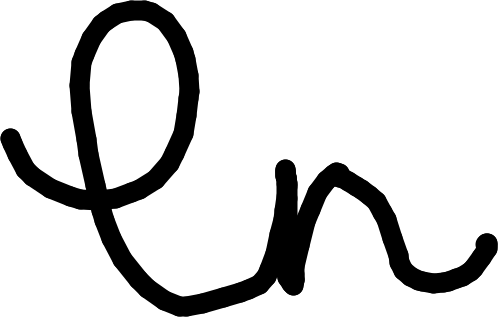
\includegraphics[height=30pt]{signature}
\vspace*{-1em}\\
\rule{3cm}{0.5pt}\\
Maria Nicolae\\
2024-05-17

\section*{Acknowledgements}
First of all, I would like to acknowledge my supervisor, Dr John Bartholomew. I thank him both for guiding and directing me throughout this project and for letting me occasionally deviate from that guidance and direction. I thank him for his patience while I was onboarding and learning the background for this project. I thank him for his hard working reviewing and giving feedback on drafts of this report as well as earlier Honours documents such as the talk and research plan. I also thank him for giving me the opportunities to attend the 2023 EQUS Annual Workshop and 2024 Quantum Australia conferences. 

Next, I would like to thank Professor Andrew Doherty for taking time out of his day to help me understand quantum input-output theory, as well as for helping me reason about unitary transformations of Rabi Hamiltonians. I would also like to thank Gargi Tyagi for our discussions on input-output theory. 

I would like to thank Dr Sahand Mahmoodian for our discussions about my biphoton generation modelling, and helping to clarifying some subtle points about the underlying physics, as well as future possibilities for the model.

I would like to thank Ben Field and John for giving me spin Hamiltonian code that helped me understand the system so that I could write my own minimal implementation of the spin Hamiltonian of ytterbium.

Finally, I would like to thank Gargi and Alice Jeffery for reading drafts of this report and giving me feedback, and Alice, Tim Newman, Ben, Gargi, John, and Elizabeth Marcellina for giving me feedback on a practice talk.

\section*{Statement of Contribution of Student}
I programmed my own implementations of the three-level transduction models in References \cite{fernandez-gonzalvo_2019} and \cite{barnett_longdell_2020}, and used these to replicate some of the plots in those references. After noticing discrepancies between and inconsistencies within those papers regarding phase conventions, I ran one of my model implementations to evaluate input and output phases, finding that only one convention produced physically sensible results.

I developed and implemented in code a model for four-level transduction, building on top of the concepts in the existing three-level transduction models. I implemented numerical methods to mitigate grid aliasing that were based on and built on top of methods in Reference \cite{barnett_longdell_2020}. I then benchmarked this model against results from experiments described in Reference \cite{bartholomew_chip_2020}, finding the model parameters corresponding to those experiments, using a mixture of theory and trial-and-error manual adjustments. My supervisor also helped refine those parameters.

I developed and implemented both steady-state and dynamical models for biphoton generation in three-level atomic systems, adapting the three-level transduction model in Reference \cite{barnett_longdell_2020} by changing indices of input and output atomic transitions, and modifying the atomic dynamics part of the model to accommodate vacuum interactions that start the generation processes into empty cavities.


\tableofcontents

\chapter{Introduction}

\section{Quantum Networking}
There are a diverse range of quantum technologies presently being researched and developed. These include quantum computing\cite{divincenzo_2000}, quantum simulation\cite{macdonell_2021}, and quantum sensing and metrology\cite{giovannetti_2004}. Quantum computing is the algorithmic processing and transformation of data encoded in the joint state space (the \textit{Hilbert space}) of multiple two-level systems (\textit{qubits}), which can offer an exponential speed advantage over classical computers on certain algorithms. Quantum simulation uses an engineered, controllable quantum system, known as a quantum simulator, to implement a Hamiltonian analogous to that of some natural or less controlled quantum system, in order to study its behaviour. Quantum sensing and metrology uses the great sensitivity of quantum systems to their environments to make measurements more precise than classical equipment can.

These systems have distinct applications from each other, but are not inherently interoperable. Additionally, all of these systems have proven challenging to scale up. \textit{Quantum networking} would alleviate both of these issues by allowing these systems to communicate quantum states between each other, rather than mere measurement outcomes as in classical networking. Quantum networking would greatly expand the joint Hilbert spaces of quantum computers and simulators, allowing them to solve larger problems, and allow them to interoperate with quantum sensors. It would also enable the use of quantum cryptography\cite{bennett_brassard_2014,yin_2016} in large, complex networks, which could enable eavesdropping to be detected, through a process analogous to the observer effect. Finally, quantum networking would enable fundamental experiments of quantum physics, such as tests of Bell's inequality, at greater scales than previously possible\cite{rosenfeld_2017}.

\section{Correlating Microwave and Optical Photons}
\begin{figure}[h]
\centering
\includetikzpicture{quantum-networking.tikz}
\caption{\label{fig:quantum_networking} Quantum networking of two distant machines using transduction (top) and biphoton generation (bottom). Measurements of the combined optical signals entangle the two machines.}
\end{figure}
Many quantum technology platforms, such as superconducting circuits and trapped ions, have energy levels separated by microwave transition frequencies, meaning that they absorb and emit microwave photons. Directly transmitting single microwave photons between quantum devices, however, is impractical. This is because bulky and expensive cooling infrastructure is needed across the entire length of the link, to mitigate thermal microwave noise and loss.

On the other hand, optical photons can much more easily be transmitted across multi-kilometre distances using optical fibres (and further if quantum repeaters\cite{briegel_1998} are used). Thermal noise is negligible for optical frequencies, even at room temperature, so no cooling is necessary. In order to use optical photons to network microwave-energy quantum systems, we would need to be able to entangle the quantum information in microwave and optical photons. This would require the use of hybrid systems that contain both optical and microwave degrees of freedom. One way to use such a hybrid system for quantum networking is \textit{transduction}, in which a transducer directly converts microwave and optical photons by absorbing one type and emitting the other type, and vice versa. Another approach is entangled microwave-optical photon pair generation (henceforth called \textit{biphoton generation} for short).

Quantum networking using these processes is illustrated in Figure \ref{fig:quantum_networking}. To entangle two distant quantum machines, one approach would be for a microwave photon to be emitted from one machine, transduced to an optical photon, and then transduced back to a microwave photon at the other end, to interact with the other machine. Another approach, using biphoton generation, would be to generate entangled pairs on either end, interact the microwave photons with the machines, and interfere and measure the optical photons at some common destination.

\section{Wave Mixing Processes}
In order for microwave and optical photons to interact through some mediating system, that system must have some nonlinearity through which \textit{wave-mixing} processes, in which frequencies mix to produce new frequencies, can occur. The simplest of these processes are second-order \textit{three-wave mixing} processes, in which three frequencies are involved. These processes include \textit{sum frequency generation} (SFG), in which two input frequencies $\omega_1$ and $\omega_2$ mix to produce a third output frequency $\omega_3 = \omega_1+\omega_2$, \textit{difference frequency generation} (DFG), in which two input frequencies mix to produce an output frequency $\omega_3 = \abs{\omega_1-\omega_2}$, and \textit{spontaneous parametric downconversion} (SPDC), in which a single input frequency $\omega_1$ produces two output frequencies $\omega_2$ and $\omega_3$ for which $\omega_2+\omega_3 = \omega_1$.

Transduction can be performed through the mixing of microwave frequencies $\omega_\mu$ and optical frequencies $\omega_o$ with an optical pump $\omega_p$; SFG $\omega_p+\omega_\mu = \omega_o$ for microwave to optical transduction and DFG $\abs{\omega_p-\omega_o} = \omega_\mu$ for optical to microwave transduction. An $\omega_\mu$ and $\omega_o$ photon pair can be generated through SPDC $\omega_p = \omega_o+\omega_\mu$. (Note that $\omega_p < \omega_o$ for transduction but $\omega_p > \omega_o$ for biphoton generation.)

\section{Hybrid Microwave-Optical Quantum Systems}
\begin{figure}[h]
\centering
    \begin{subfigure}{0.32\textwidth}
    \centering
    \includetikzpicture{chi-2.tikz}
\end{subfigure}
\begin{subfigure}{0.32\textwidth}
    \centering
    \includetikzpicture{optomechanics.tikz}
\end{subfigure}
\begin{subfigure}{0.32\textwidth}
    \centering
    \includetikzpicture{hybrid-atomic-system.tikz}
\end{subfigure}
\caption{\label{fig:hybrid_systems} Hybrid microwave-optical platforms illustrated, including $\chi^{(2)}$-nonlinear dielectric media (left), optomechanical systems (middle), and atomic energy levels (right).}
\end{figure}
Many different hybrid systems and processes have been proposed and experimentally studied for use in transduction and biphoton generation. One example of such systems are dielectric media with secord-order nonlinear polarisabilities \cite{rueda_2016,rueda_2019,sahu_2023} ($\chi^{(2)} \neq 0$). In these media, incident electromagnetic waves create time-varying polarisation in the material at new frequencies that are then emitted, giving rise to three-wave mixing. Another example is optomechanical systems\cite{bochmann_2013,higginbotham_2018}, in which a mechanical resonator simultaneously constitutes a mirror in an optical resonant cavity and a capacitor in a microwave resonator. This results in coupling between the optical, mechanical, and microwave modes. Yet another platform is atoms with both microwave and optical transitions between their energy levels\cite{staudt_2012,probst_2013}, in which both types of photons can interact with atomic transitions. Reviews of the various systems can be found at References \cite{lambert_2020,lauk_2020}. My project focuses on atomic systems in particular.

\section{Hybrid Atomic Systems}
\begin{figure}[h]
\centering
\includetikzpicture{lambda-and-v-systems.tikz}
\caption{\label{fig:lambda_and_v_systems} Transduction in a \textLambda-system (left) and V-system (middle), and biphoton generation in a \textLambda-system (right).}
\end{figure}

\noindent Atoms can be used for transduction by working in a three-level system consisting of two levels separated by a microwave transition and a third level separated from the other two by optical transitions. This can either be a \textit{\textLambda-system}, in which the $\ket{1}$ and $\ket{2}$ levels are microwave-separated, or a \textit{V-system}, in which $\ket{2}$ and $\ket{3}$ are microwave-separated\footnote{\textLambda-systems and V-systems are named as such because the two optical transitions form diagrams resembling those glyphs.}. To perform transduction in a \textLambda-system, $\ket{2}\leftrightarrow\ket{3}$ is pumped so that absorption of a microwave photon by the $\ket{1}\to\ket{2}$ transition results in coherence between the $\ket{1}$ and $\ket{3}$ levels and ultimately the emission of an optical photon from the $\ket{3}\to\ket{1}$ transition, and vice-versa. In a V-system, $\ket{1}\to\ket{2}$ is pumped, microwave signals interact with the $\ket{2}\leftrightarrow\ket{3}$ transition, and optical signals interact with $\ket{1}\leftrightarrow\ket{3}$. Biphoton generation can be performed by pumping $\ket{1}\to\ket{3}$ to obtain continuous output of $\ket{3}\to\ket{2}$ and $\ket{2}\to\ket{1}$ photon pairs. These processes are illustrated in Figure \ref{fig:lambda_and_v_systems}.

\begin{figure}[h]
\centering
\input{inhomogeneous-broadening.pgf}
\caption{\label{fig:inhomogeneous_broadening} Inhomogeneous broadening of an atomic ensemble's absorption spectrum. The individual atoms have absorption spectra (grey filled curves) that are slightly shifted from each other, resulting in an overall ensemble absoption spectrum (dashed line) that is broader than the individual atom spectrum.}
\end{figure}

Atoms can be used in quantum technology as electromagnetically trapped ions or neutral atoms, or as constituents of crystals, with the latter being the focus of my project. Atoms in crystals are more miniaturisable and therefore scalable than trapped atoms because they do not need trapping infrastructure; confinement is provided by the crystal. Scaling is desirable because the more atoms are used, the stronger their collective interactions with the microwave and optical signals are. However, atomic ensembles in crystals are subject to \textit{inhomogeneous broadening} of the collective spectral line shapes, compared to individual atoms.

Let the absorption spectrum of a single atom around its transition frequency $\omega_0$ (the \textit{homogeneous} lineshape) be $\alpha_S(\omega-\omega_0)$. The absorption spectrum of $N$ atoms of the same species, if all atoms had the same transition frequency, would simply be
\begin{equation}
    \alpha_E(\omega) = N\alpha_S(\omega-\omega_0).
\end{equation}
However, in a crystal, every atom has its own slightly different transition frequency $\omega_0$. This is because each atom has a slightly different local electromagnetic field due to strain and defects in the crystal, which shift the atomic energy levels via effects such as the Stark and Zeeman effects, by a different amount for each atom. Given that the atomic transition frequencies are distributed with probability density function (PDF) $p(\omega_0)$, the absorption spectrum of an $N$-atom ensemble (the \textit{inhomogeneous} lineshape) is
\begin{equation}
    \label{eq:inhomogeneous_convolution}
    \alpha_E(\omega) = N \int_0^\infty \alpha_S(\omega-\omega_0)p(\omega_0)\:d\omega_0 = N\alpha_S * p.
\end{equation}
This is at least as wide as the homogeneous line width, and is usually much wider.

\subsection{Rare Earths}
Of all atomic species one could use for hybrid systems, rare earths are a leading candidate. Their states have long coherence times, such as nuclear spin coherence times longer than $\qty{1}{\second}$ in Er\textsuperscript{3+}\cite{ranvcic_2018} and up to 6 hours in Eu\textsuperscript{3+}\cite{zhong_2015}, and electronic coherence times of $\qty{4}{\milli\second}$ in Er\textsuperscript{3+}\cite{bottger_2009}. Rare earths also have narrow inhomogeneous linewidths\cite{vleck_1937}, $\unit{\mega\hertz}$ for microwave transitions and hundreds of $\unit{\mega\hertz}$ for optical transitions. Both of these properties are the result of the full $5s$ and $5p$ electron shells of rare earths having larger radii than their $4f$ valence shells, which shields the latter from the external environment\cite{wybourne_book}. Erbium in particular has an optical transition frequency in the infrared telecommunications band which is attenuated least by optical fibres, making it well-suited for long-distance communication and networking applications.

\section{\label{sec:quantum_theory}Background Quantum Theory}
This section explains the quantum-mechanical formalisms that are used throughout the remainder of the thesis. This begins with \textit{second quantisation}, the quantum description of light and systems that interact with light (\textit{quantum emitters}), and then describes those interactions as exchanges of energy quanta, and a semiclassical approximation thereof. Then, the theory of inputs and outputs of quantum systems is presented. Finally, a formalism for quantum decoherence is presented; due to this being a stochastic phenomenon, this formalism is expressed in terms of probabilistic mixtures of quantum states.

\subsection{Second Quantisation}
In the formalism of \textit{second quantisation}, quantum systems are analysed as being composed of components (\textit{modes}) which are occupied by energy quanta. These modes have Hamiltonians of the form
\begin{equation}
    \hbar\omega_0\hat{n} \label{eq:second_quantisation_hamiltonian}
\end{equation}
where
\begin{equation}
    \hat{n} = \sum_n n\ket{n}\bra{n} \label{eq:number_operator_definition}
\end{equation}
is the observable for the number of energy quanta in the mode, and $\hbar\omega_0$ is the energy quantum.

For a \textit{bosonic} mode, the sum in Equation \ref{eq:number_operator_definition} is over $n = 0, 1, 2, \dots$, i.e. an arbitrarily large number of quanta can occupy the mode. An electromagnetic cavity mode is a bosonic mode, with the energy quanta being photons. For a \textit{fermionic} mode, only one quantum can occupy it, and $n=0,1$ only. The fermionic $\ket{0}$ and $\ket{1}$ states are sometimes alternatively denoted $\ket{g}$ (\textit{ground}) and $\ket{e}$ (\textit{excited}) respectively. A two-level quantum emitter is a fermionic mode, and the level pairs of multi-level systems like atoms can be modelled as fermionic modes.

\subsubsection{Ladder Operators}
The \textit{number operator}
\begin{equation}
\hat{n}=\hat{c}^\dagger\hat{c} \label{eq:number_operator_from_ladders}
\end{equation}
is composed of a \textit{lowering operator} $\hat{c}$ and a \textit{raising} operator\footnote{Alternatively, \textit{annihilation} and \textit{creation} operator respectively} $\hat{c}^\dagger$. These ladder operators act on number states by lowering or raising them respectively to adjacent number states. Specifically, the bosonic ladder operators act on number states by
\begin{equation}
    \hat{a}\ket{n} = \sqrt{n}\ket{n-1}, \quad \hat{a}^\dagger\ket{n} = \sqrt{n+1}\ket{n+1},
\end{equation}
and the fermionic ladder operators are
\begin{equation}
    \hat{\sigma} = \ket{0}\bra{1}, \quad \hat{\sigma}^\dagger = \ket{1}\bra{0};
\end{equation}
$\hat{c}$ in Equation \ref{eq:number_operator_from_ladders} is any one of $\hat{a}$ or $\hat{\sigma}$. These operators have commutation relations\footnote{Here, unlike in Equation \ref{eq:second_quantisation_hamiltonian}, $\hbar=1$ is used and $\hbar$ is dropped accordingly. The same will be done in the remainder of this thesis.}
\begin{equation}
    [\hat{a}, \hat{a}^\dagger] = \hat{\mathds{1}}, \quad [\hat{\sigma}, \hat{\sigma}^\dagger] = \hat{\mathds{1}} - 2\hat{\sigma}^\dagger\hat{\sigma}.
\end{equation}
As the notation suggests, ladder operators are Hermitian conjugates of each other, and the lowering operator, by convention, is the one represented without a dagger.

\subsection{Light-Matter Interactions}

\subsubsection{Quantum Model}
In the language of second quantisation, light-matter interactions are described in terms of an electromagnetic cavity with lowering operator $\hat{a}$ and a two-level quantum emitter with lowering operator $\hat{\sigma}$. Here I consider light-matter interactions through the dipole interaction, which, for the example of an electric dipole, is represented by a Hamiltonian
\begin{equation}
    \hat{H} = \hat{H}_\text{light} + \hat{H}_\text{emitter} - \vhat{d} \cdot \vhat{E}.
\end{equation}
$\vhat{d}$ is the dipole moment operator of the emitter, and can therefore be expressed in terms of $\hat{\sigma}$, and $\vhat{E}$ is the electric field operator, which can be expressed in terms of $\hat{a}$. Making appropriate approximations\footnote{The \textit{rotating wave approximation}} and writing the result out in terms of mode operators yields the \textit{Jaynes-Cummings Hamiltonian}\cite{jaynes_cummings_1963,gerry_knight_book}
\begin{equation}
    \hat{H}_\text{JC} = \omega_r\hat{a}^\dagger\hat{a} + \omega_a\hat{\sigma}^\dagger\hat{\sigma} + g(\hat{a}\hat{\sigma}^\dagger + \hat{a}^\dagger\hat{\sigma}). \label{eq:jaynes_cummings_hamiltonian}
\end{equation}
Here, $\omega_r$ is the resonant frequency of the cavity, $\omega_a$ is the transition frequency of the emitter, and $g$ is a constant representing the strength of the interaction. The terms $\hat{a}\hat{\sigma}^\dagger$ and $\hat{a}^\dagger\hat{\sigma}$ that are scaled by $g$ represent the interaction itself as the transfer of energy quanta between the cavity and the emitter. Because this interaction is through the dipole mechanism, the interaction strength is proportional to
\begin{equation}
    g \propto \bra{g} \hat{d}_{\parallel} \ket{e} \label{eq:g_dipole_moment}
\end{equation}
the component of the dipole moment matrix element parallel to the light polarisation.

\subsubsection{\label{ssubs:semiclassical_light_matter}Semiclassical Approximation and Rabi Frequencies}
A unitary transformation of Equation \ref{eq:jaynes_cummings_hamiltonian} eliminates the cavity energy term to obtain
\begin{equation}
    \hat{H} = \omega_a\hat{\sigma}^\dagger\hat{\sigma} + g\hat{a}e^{-i\omega_rt} \hat{\sigma}^\dagger + g\hat{a}^\dagger e^{i\omega_rt} \hat{\sigma}.
\end{equation}
To form a semiclassical approximation, the cavity operator $\hat{a}$ is replaced with a complex number $\alpha$ that represents the amplitude and phase of a `classical-like' cavity state\footnote{Known as a \textit{coherent state}; see Reference \cite{gerry_knight_book}.}, scaled so that $\abs{\alpha}^2 = \angbr{\hat{n}}$ resulting in the semiclassical \textit{mean-field} model in \cite{walls_milburn_book}, a Hamiltonian which, in the $(\ket{g}, \ket{e})$ basis of the emitter, is
\begin{equation}
    \hat{H} =
    \begin{bmatrix}
        0 & g\alpha^* e^{i\omega_rt}\\
        g\alpha e^{-i\omega_rt} & \omega_a
    \end{bmatrix}. \label{eq:two_level_time_dependent_rabi_hamiltonian}
\end{equation}
This represents the dipole interaction between a quantum emitter and a classical oscillating electromagnetic field in terms of the \textit{Rabi frequency} $\Omega = g\alpha$. More specifically, for the example of an electric dipole,
\begin{equation}
    \Omega = \frac{\bra{g}\vhat{d}\ket{e} \cdot \vec{\mathcal{E}}_0}{\hbar} \label{eq:rabi_frequency_dipole_moment}
\end{equation}
where $\vec{\mathcal{E}}_0$ is the complex amplitude of the electric field. This model therefore also applies to emitters driven by waveguides or free-space light beams, for some $\Omega$ that has no interpretation as a $g\alpha$. A unitary transformation of Equation \ref{eq:two_level_time_dependent_rabi_hamiltonian} gives a time-independent Hamiltonian
\begin{equation}
    \hat{H} =
    \begin{bmatrix}
        0 & \Omega^*\\
        \Omega & \omega_a-\omega_r
    \end{bmatrix}. \label{eq:two_level_time_independent_rabi_hamiltonian}
\end{equation}
Furthermore, Equation \ref{eq:two_level_time_dependent_rabi_hamiltonian} can be extended quite simply to driven multi-level systems: for energy levels indexed by $k$ and drives indexed by $\ell$,
\begin{equation}
    \hat{H} = \sum_{k} \omega_k\hat{\sigma}_{kk} + \sum_{\ell} \left(\Omega_\ell e^{i\omega_\ell t} \hat{\sigma}_{i_\ell j_\ell} + \Omega^*_\ell e^{-i\omega_\ell t} \hat{\sigma}_{j_\ell i_\ell}\right) \label{eq:multi_level_time_dependent_rabi_hamiltonian}
\end{equation}
where $\hat{\sigma}_{ij} = \ket{i}\bra{j}$ are unit matrices and $i_\ell j_\ell$ are the transitions driven by drive $\ell$.

\subsection{\label{subs:heisenberg_picture}The Heisenberg Picture}
The \textit{Heisenberg picture} of quantum mechanics is a formulation of quantum mechanics in which operators evolve in time, but state vectors (kets) are static, representing initial conditions. This is in opposition to the \textit{Schr\"{o}dinger picture}. Operators in the Heisenberg picture obey the \textit{Heisenberg equation}\cite{sakurai_book}
\begin{equation}
    \frac{d\hat{A}}{dt} = -i[\hat{A}, \hat{H}].
\end{equation}
When forming semiclassical approximations that replace light operators with amplitudes, such as in Subsection \ref{ssubs:semiclassical_light_matter}, the Heisenberg equation of a light operator becomes the differential equation of the amplitude.

\subsubsection{\label{ssubs:input_output_theory}Langevin Equations and Input-Output Theory}
If we have some system, with Hamiltonian $\hat{H}_\text{sys}$ that is coupled through an operator $\hat{c}$ to a waveguide or transmission line, \textit{input-output theory}\cite{gardiner_collett_1985} provides a quantum model of such a system, which includes the dynamics of some (not necessarily bosonic) system operator $\hat{a}$ expressed in terms of modified Heisenberg equation, known as a \textit{Langevin equation},
\begin{equation}
    \frac{d\hat{a}}{dt} = -i[\hat{a}, \hat{H}_\text{sys}] + [\hat{a}, \hat{c}^\dagger]\left(-\frac{\gamma}{2}\hat{c} + \sqrt{\gamma}\hat{b}_\text{in}(t)\right) + \left(\frac{\gamma}{2}\hat{c}^\dagger - \sqrt{\gamma}\hat{b}_\text{in}^\dagger(t)\right)[\hat{a}, \hat{c}]. \label{eq:general_langevin_equation}
\end{equation}
Here, $\hat{b}_\text{in}(t)$ is a bosonic-like operator representing the input from the waveguide into the system at time $t$, and $\gamma$ is the rate of energy loss from $\hat{c}$ into the waveguide. A similar output operator is
\begin{equation}
    \hat{b}_\text{out}(t) = -\hat{b}_\text{in}(t) + \sqrt{\gamma}\hat{c}.
    \label{eq:input_output_theory_output}
\end{equation}
The operators $\hat{b}_\text{in}(t)$ and $\hat{b}_\text{out}(t)$ at one time and at another time correspond to separate modes, and should not be interpreted as any sort of time evolution. Loosely speaking, we can think of these operators as representing $\delta$-function pulses that arrive at the system at time $t$, which can be integrated over to form arbitrary signals.

\subsection{Density Matrices and the Master Equation}
A \textit{density matrix}\cite{breuer_book} for a system is an operator which describes the probability distribution of states in that system, distinguishing `classical' probability from quantum superpositions. For states $\ket{\psi_k}$ with probabilities $p_k$, the density matrix is
\begin{equation}
    \hat{\rho} = \sum_k p_k \ket{\psi_k}\bra{\psi_k}. \label{eq:density_matrix_definition}
\end{equation}
In the Schr\"{o}dinger picture, density matrices evolve according to the \textit{Master equation}\footnote{Alternatively, the \textit{Lindblad equation}}
\begin{equation}
    \frac{d\hat{\rho}}{dt} = -i[\hat{H}, \hat{\rho}].
\end{equation}
The expectation value of an operator $\hat{O}$ can be calculated from a density matrix $\hat{\rho}$ as
\begin{equation}
    \angbr{\hat{O}} = \tr(\hat{\rho}\hat{O}), \label{eq:density_matrix_expectation_value}
\end{equation}
which, for a density matrix of the form in Equation \ref{eq:density_matrix_definition}, is the weighted sum of the expectation value for all $\ket{\psi_k}$ states
\begin{equation}
    \angbr{\hat{O}} = \sum_k p_k \bra{\psi_k}\hat{O}\ket{\psi_k}.
\end{equation}

\subsubsection{Density Matrices and Quantum Decoherence}
Consider the density matrix of a two-level system. A pure ground state $\ket{0}$ has density matrix
\begin{equation}
    \hat{\rho} = \ket{0}\bra{0} =
    \begin{bmatrix}
        1 & 0\\
        0 & 0
    \end{bmatrix},
\end{equation}
whereas an even probabilistic mixture of $\ket{0}$ and $\ket{1}$ has density matrix
\begin{equation}
    \hat{\rho} = \frac{1}{2}\left(\ket{0}\bra{0}+\ket{1}\bra{1}\right) =
    \begin{bmatrix}
        \frac{1}{2} & 0\\
        0 & \frac{1}{2}
    \end{bmatrix}.
\end{equation}
This demonstrates that the diagonal elements of a density matrix represent probabilities of states. Indeed, $\tr\hat{\rho}=1$. The even superposition $\ket{\psi} = \frac{1}{\sqrt{2}}\left(\ket{0}+\ket{1}\right)$ has density matrix
\begin{equation}
    \hat{\rho} = \ket{\psi}\bra{\psi} =
    \begin{bmatrix}
        \frac{1}{2} & \frac{1}{2}\\
        \frac{1}{2} & \frac{1}{2}
    \end{bmatrix},
\end{equation}
which demonstrates that the off-diagonal elements represent \textit{coherences} between states. That is to say, they distinguish between superpositions and classical probabilities.

Density matrices are a useful formalism for expressing quantum decoherence. The two types of decoherence in quantum systems are \textit{depolarisation} and \textit{dephasing}. Depolarisation is unwanted transitions between states, which includes transitions to lower-energy states (\textit{relaxation}) as well as unwanted excitations to higher-energy states. In a density matrix, this is represented by changes in the diagonal elements. Dephasing is drift in relative phase between states, caused by fluctuations in the energy levels. This is represented by decreases in the magnitudes of the off-diagonal elements. The dynamics of decoherence can be represented by additional terms in the Master equation. For decoherence resulting from the coupling of operators $\hat{A}_k$ to the environment, with rates $\gamma_k$, the Master equation becomes
\begin{equation}
    \frac{d\hat{\rho}}{dt} = -i[\hat{H}, \hat{\rho}] + \sum_k \frac{\gamma_k}{2}\left(2\hat{A}_k\hat{\rho}\hat{A}_k^\dagger - \hat{A}_k^\dagger\hat{A}_k\hat{\rho} - \hat{\rho}\hat{A}_k^\dagger\hat{A}_k\right).
\end{equation}
In both the original and prior modelling work presented in this thesis, density matrices are used to represent the states of atoms, but not cavities. This is because cavities do not dephase, only depolarise by gaining and losing photons, and so the input-output formalism of Subsection \ref{ssubs:input_output_theory} is better suited.

\section{Outline of Thesis}
This thesis is structured as follows. Chapter \ref{ch:prior_transduction} mostly presents prior work on both numerical and analytical modelling for atomic ensemble based microwave-optical transduction, that the original work in this thesis builds from. At the end of that chapter, in Section \ref{sec:rho_ji_vs_ij}, it describes original work on analysing phase conventions and relations in that model. Chapter \ref{ch:four_level_transduction} describes original numerical modelling for transduction in four-level atomic systems. This model computes transduction signal strengths, and thereby conversion efficiencies. The chapter also compares model and experimental results. Chapter \ref{ch:biphoton_generation} describes numerical modelling for the pair generation rate resulting from biphoton generation in three-level atomic systems. Finally, Chapter \ref{ch:conclusion} concludes the thesis.

\chapter{\label{ch:prior_transduction}Prior Work on Transduction Modelling}

\begin{figure}[h]
\centering
\includetikzpicture{atoms-in-cavity.tikz}
\caption{\label{fig:3lt_diagram} An illustration of a crystal in a cavity, with signals entering and exiting the cavity.}
\end{figure}

\noindent In this chapter, I review some existing modelling work\cite{williamson_2014,fernandez-gonzalvo_2019,barnett_longdell_2020} for microwave-optical quantum transduction using atomic ensembles in microwave and optical cavities. This prior work focuses on atoms in cavities rather than in free space, because cavity-based systems promise to be more efficient because of stronger light-matter interactions in cavities due to concentrated electromagnetic field. To begin, I present a fully quantum model for three-level atoms in cavities in Section \ref{sec:3lt_quantum_model}, and then in later sections, I review the semiclassical models of References \cite{williamson_2014,fernandez-gonzalvo_2019,barnett_longdell_2020}, and discuss the approximations made in those models. In Section \ref{sec:rho_ji_vs_ij}, I investigate relations between input and output phases in these models, and find that there is a physically sensible phase relation only if a particular modification is made to the model. The phases of optical photons can be used to encode quantum information, and so accurate predictions of phase are important to such applications. Notation used here may differ from that of the original sources.

\section{\label{sec:3lt_quantum_model}Quantum Model}
A fully quantum model for such a system is the Jaynes-Cummings-like Hamiltonian\cite{barnett_longdell_2020}
\begin{equation}
\label{eq:atoms_in_cavities_full_hamiltonian}
    \hat{H} = \hat{H}_\text{cavities} + \sum_{k=1}^{N} \hat{H}_{\text{atom},k} + \sum_{k=1}^{N} \hat{H}_{\text{int},k}
\end{equation}
where $N$ is the total number of active atoms and $k$ is an index over the atoms. The Hamiltonian of the cavities is
\begin{equation}
    \hat{H}_\text{cavities} = \delta_{co} \hat{a}^\dagger\hat{a} + \delta_{c\mu} \hat{b}^\dagger\hat{b}
\end{equation}
where $\hat{a}$ and $\hat{b}$ are the lowering operators of the optical and microwave cavity modes respectively, and $\delta_{co} = \omega_{co} - \omega_o$ and $\delta_{c\mu} = \omega_{c\mu} - \omega_\mu$ are the detunings of the optical and microwave signals respectively from the resonant frequencies of the cavities. The other two components of Equation \ref{eq:atoms_in_cavities_full_hamiltonian} depend on whether the three-level system being used is a \textLambda-system or a V-system. The atom Hamiltonian, with both cases explicitly written out, is
\begin{equation}
    \hat{H}_{\text{atom},k} =
    \begin{cases}
        \delta_{\mu,k} \hat{\sigma}_{22,k} + \delta_{p,k} \hat{\sigma}_{33,k} & \text{\textLambda-system}\\
        \delta_{o,k} \hat{\sigma}_{22,k} + \delta_{p,k} \hat{\sigma}_{33,k} & \text{V-system}
    \end{cases}.
\end{equation}
$\hat{\sigma}_{ij,k} = \ket{i_k}\bra{j_k}$ are atomic unit matrices, $\delta_{o,k} = \omega_{13,k} - \omega_o$ is the detuning of the optical signal from the $\ket{1}\leftrightarrow\ket{3}$ transition frequency, and $\delta_{\mu,k}$ and $\delta_{p,k}$ are the detunings of the microwave and pump signals respectively from their corresponding atomic transition frequencies. These transition frequencies are different for each atom due to inhomogeneous broadening. By conservation of energy, $\delta_{\mu,k} + \delta_{p,k} = \delta_{o,k}$, and so, even though we only directly control the frequency of the two inputs, we always know the frequency of the output. The interaction Hamiltonian is
\begin{equation}
    \hat{H}_{\text{int},k} = \Omega_{p,k}\hat{\sigma}_{i_p j_p,k} + g_{o,k}\hat{a}\hat{\sigma}_{31,k} + g_{\mu,k}\hat{b}\hat{\sigma}_{i_\mu j_\mu,k} + \text{h.c.}
\end{equation}
where $\Omega_{p,k}$ is the pump Rabi frequency on atom $k$, $g_{o,k}$ and $g_{\mu,k}$ are the coupling strengths of atom $k$ to the optical and microwave cavities respectively, and $i_p$ and $j_p$ ($i_\mu$ and $j_\mu$) are the lower and upper atomic levels respectively of the transition corresponding to the pump (microwave) signal.

The cavity Langevin equations for this system, which include damping and signal input-output, are
\begin{align}
    \frac{d\hat{a}}{dt} &= -i\delta_{co}\hat{a} - i\sum_{k=1}^{N} g_{o,k}^*\hat{\sigma}_{13,k} - \frac{\gamma_{oi}+\gamma_{oc}}{2}\hat{a} + \sqrt{\gamma_{oc}}\hat{a}_\text{in}(t) \label{eq:optical_cavity_quantum_langevin}\\
    \frac{d\hat{b}}{dt} &= -i\delta_{c\mu}\hat{b} - i\sum_{k=1}^{N} g_{\mu,k}^*\hat{\sigma}_{i_\mu j_\mu,k} - \frac{\gamma_{\mu i}+\gamma_{\mu c}}{2}\hat{b} + \sqrt{\gamma_{\mu c}}\hat{b}_\text{in}(t)
\end{align}
where $\gamma_{oi}$ and $\gamma_{oc}$ ($\gamma_{\mu i}$ and $\gamma_{\mu c}$) are the energy loss rates of the optical (microwave) cavity through intrinsic damping and coupling to the input-output channel respectively. The output operators are, in analogy with Equation \ref{eq:input_output_theory_output},
\begin{align}
    \hat{a}_\text{out}(t) &= -\hat{a}_\text{in}(t) + \sqrt{\gamma_{oc}}\hat{a}(t) \label{eq:input_output_relation_a}\\
    \hat{b}_\text{out}(t) &= -\hat{b}_\text{in}(t) + \sqrt{\gamma_{\mu c}}\hat{b}(t) \label{eq:input_output_relation_b}.
\end{align}

\section{\label{sec:adiabatic_elimination}Adiabatic Elimination of the Atomic Dynamics}
\noindent The fully quantum model is intractable to solve exactly. One approach to simplifying the model into something tractable is that of Williamson et.\ al.\ (2014) \cite{williamson_2014}. By assuming that the atom-signal detunings are large ($\abs{\delta_{o,k}} \gg \abs{g_{o,k}}$, $\abs{\delta_{\mu,k}} \gg \abs{g_{\mu,k}}$, and $\abs{\delta_{o,k}\delta_{\mu_k}} \gg \abs{\Omega_{p,k}}^2$), we can approximate the indirect interaction of the microwave and optical cavities as a direct interaction, \textit{adiabatically eliminating}\cite{brion_2007} the atomic dynamics. This gives an effective interaction Hamiltonian for the system
\begin{equation}
    \hat{H}_\text{eff} = S\hat{a}^\dagger\hat{b} + S^*\hat{a}\hat{b}^\dagger
\end{equation}
where the effective interaction strength is
\begin{equation}
    S = \sum_{k=1}^{N} \frac{\Omega_{p,k}g_{\mu,k}g_{o,k}^*}{\delta_{o,k}\delta_{\mu,k}}.
\end{equation}
Note that this is the same Hamiltonian as for two cavities that share a mirror, with the transduction process being analogous to photons passing through the shared mirror. The cavity Langevin equations are then
\begin{align}
    \frac{d\hat{a}}{dt} &= -iS\hat{b} - \frac{\gamma_{oc}}{2}\hat{a} + \sqrt{\gamma_{oc}}\hat{a}_\text{in}(t)\\
    \frac{d\hat{b}}{dt} &= -iS^*\hat{a} - \frac{\gamma_{\mu c}}{2}\hat{b} + \sqrt{\gamma_{\mu c}}\hat{b}_\text{in}(t);
\end{align}
this model further assumes that all loss in the cavities is through the input-output channels, i.e. $\gamma_{oi} = \gamma_{\mu i} = 0$. In the steady state of the cavities, the conversion efficiency (in both directions) can be found analytically to be
\begin{equation}
    \eta = \abs{\frac{4iS\sqrt{\gamma_{oc}\gamma_{\mu c}}}{4\abs{S}^2+\gamma_{oc}\gamma_{\mu c}}}^2.
\end{equation}

\section{Semiclassical Cavity and Atomic Master Equation Steady States}
A less simplistic model, one which must be solved numerically rather than analytically, is that of Fernandez-Gonzalvo et.\ al.\ (2019) \cite{fernandez-gonzalvo_2019}. That paper only explicitly describes \textLambda-systems, but the generalisation to V-systems is straightforward. In this model, the atom-cavity interaction is replaced with semiclassical (Rabi) drives in the atom Hamiltonian
\begin{equation}
    \hat{H}_{\text{atom},k} =
    \begin{bmatrix}
        0 & \Omega_{\mu,k}^* & \Omega_{o,k}^*\\
        \Omega_{\mu,k} & \delta_{\mu,k} & \Omega_{p,k}^*\\
        \Omega_{o,k} & \Omega_{p,k} & \delta_{p,k}
    \end{bmatrix}
\end{equation}
where $\Omega_{\mu,k}$ and $\Omega_{o,k}$ are the Rabi frequencies of the driving that results from coupling to the microwave and optical cavities respectively. With $\alpha$ as the semiclassical amplitude of the optical cavity, $\Omega_{o,k} = g_{o,k}\alpha$. However, we do not treat the microwave cavity similarly, and instead assume that its amplitude is large enough that atomic absorption and emission is negligible, and so disregard the dynamical details of $\Omega_{\mu,k}$, setting it to be some constant value.

To handle the atomic dynamics, we use the Master equation
\begin{equation}
    \label{eq:three_level_atom_master_equation}
    \frac{d\hat{\rho}_k}{dt} =: \mathcal{L}_k\hat{\rho}_k = -i[\hat{H}_{\text{atom},k}, \hat{\rho}_k] + \mathcal{L}_{\text{dec},k}\hat{\rho}_k
\end{equation}
with decoherence operator
\begin{equation}
\label{eq:three_level_atom_loss_operator}
\begin{split}
    \mathcal{L}_{\text{dec},k}\hat{\rho}_k &= \mathcal{L}_{12,k}\hat{\rho}_k + \mathcal{L}_{13,k}\hat{\rho}_k + \mathcal{L}_{23,k}\hat{\rho}_k + \mathcal{L}_{2d,k}\hat{\rho}_k + \mathcal{L}_{3d,k}\hat{\rho}_k\\
    \mathcal{L}_{ij,k}\hat{\rho}_k &=
    \begin{cases}
        \begin{split}
            &\frac{\gamma_{ij}(n_{ij,k}+1)}{2} \left(2\hat{\sigma}_{ij,k}\hat{\rho}_k\hat{\sigma}_{ji,k} - \hat{\rho}_k\hat{\sigma}_{jj,k} - \hat{\sigma}_{jj,k}\hat{\rho}_k\right)\\
            &+ \frac{\gamma_{ij}n_{ij,k}}{2} \left(2\hat{\sigma}_{ji,k}\hat{\rho}_k\hat{\sigma}_{ij,k} - \hat{\rho}_k\hat{\sigma}_{ii,k} - \hat{\sigma}_{ii,k}\hat{\rho}_k\right)
        \end{split}
        & i=1,j=2\\
        \frac{\gamma_{ij}}{2} \left(2\hat{\sigma}_{ij,k}\hat{\rho}_k\hat{\sigma}_{ji,k} - \hat{\rho}_k\hat{\sigma}_{jj,k} - \hat{\sigma}_{jj,k}\hat{\rho}_k\right) & \text{otherwise}
    \end{cases}\\
    \mathcal{L}_{id,k}\hat{\rho}_k &= \frac{\gamma_{id}}{2} \left(2\hat{\sigma}_{ii,k}\hat{\rho}_k\hat{\sigma}_{ii,k} - \hat{\rho}_k\hat{\sigma}_{ii,k} - \hat{\sigma}_{ii,k}\hat{\rho}_k\right).
\end{split}
\end{equation}
$\gamma_{2d}$ and $\gamma_{3d}$ are the dephasing rates of levels $\ket{2}$ and $\ket{3}$ respectively with level $\ket{1}$, and $\gamma_{12,k}$, $\gamma_{13}$, and $\gamma_{23}$ are the relaxation rates via the indicated transitions. $n_{12,k}$ is the mean thermal excitation count at $\omega_{12,k}$, as per the Bose-Einstein distribution, which is approximately zero for all other transition frequencies. For this transition,
\begin{equation}
    \gamma_{12,k} = \frac{1}{\tau_{12}} \frac{1}{n_{12}+1}
\end{equation}
where $\tau_{12}$ is the relaxation lifetime, whereas the other transitions follow the simpler $\gamma_{ij} = 1/\tau_{ij}$.

$\alpha$ evolves in time according to a semiclassical approximation of Equation \ref{eq:optical_cavity_quantum_langevin}, in which $\hat{a}$ is, of course, replaced with $\alpha$, and the $\hat{\sigma}_{ij,k}$ operators in the atomic interaction terms are replaced with $\rho_{ij,k}$ to give
\begin{equation}
    \label{eq:semiclassical_optical_cavity_langevin}
    \frac{d\alpha}{dt} = -i\delta_{co}\alpha -i\sum_{k=1}^{N} g_{o,k}^* \rho_{13,k} - \frac{\gamma_{oi}+\gamma_{oc}}{2}\alpha + \sqrt{\gamma_{oc}}\alpha_\text{in}.
\end{equation}

\subsection{\label{subs:steady_states}Steady States}
Despite this model being much smaller than the fully quantum model, operators having been replaced with complex numbers, it is still intractable to solve the time evolution of, because it requires $N$ density matrices to be stored in memory. Finding steady states, however, is tractable with a few further simplifications. Let $\hat{\rho}_{k,SS}(\alpha)$ be the steady state of the density matrix of atom $k$ given an optical cavity amplitude $\alpha$, which is found by solving the linear system in Equation \ref{eq:three_level_atom_master_equation}. We can drop the $k$ index by including as function arguments all atom variables to obtain $\hat{\rho}_{SS}(\Omega_{p,k}, g_{o,k}, \alpha, \Omega_{\mu,k}, \delta_{o,k}, \delta_{\mu,k}, \omega_{12,k})$. If we assume that all atoms have the same coupling strengths and Rabi frequencies, $\hat{\rho}_{SS}$ varies only with $\alpha$ and the inhomogeneous shifts of each atom. This allows us to replace the sum in Equation \ref{eq:semiclassical_optical_cavity_langevin} with an integral over the inhomogeneous distribution, of the form in Equation \ref{eq:inhomogeneous_convolution}
\begin{equation}
    \label{eq:optical_cavity_steady_state_equation}
    \frac{d\alpha}{dt} = -i\delta_{co}\alpha -iNg_o^* \iint \rho_{13,SS}(\alpha, \delta_{12}, \delta_{23}) p(\delta_{12}, \delta_{23})\:d\delta_{12}d\delta_{23} - \frac{\gamma_{oi}+\gamma_{oc}}{2}\alpha + \sqrt{\gamma_{oc}}\alpha_\text{in}.
\end{equation}
Here, $\delta_{ij} = \omega_{ij} - \omega'_{ij}$ is the inhomogeneous shift of an atomic transition frequency $\omega_{ij}'$ from some `nominal' transition frequency $\omega_{ij}$, and $p(\delta_{12}, \delta_{23})$ is the PDF of those shifts. A value of $\alpha$ for which Equation \ref{eq:optical_cavity_steady_state_equation} is zero, i.e.\ a steady state, can be found using numerical root-finding, in which each iterative step involves evaluating the integral over the inhomogeneous distribution using some numerical quadrature scheme.

\subsection{\label{subs:barnett_longdell_development}Further Development by Barnett and Longdell (2020)}
Barnett and Longdell (2020) \cite{barnett_longdell_2020} further developed this model by including the dynamics of both cavities, with a semiclassical microwave cavity amplitude $\beta$ from which the microwave Rabi frequency $\Omega_\mu = g_\mu\beta$ derives. Additionally, the assumption that all atoms have equal interaction strengths was replaced with the assumption that $N_o \leq N$ atoms have equal $g_o$ and $N_\mu$ atoms have equal $g_\mu$, with the remaining atoms not interacting with those cavities at all, due to being outside the mode volume. Put together, this replaces Equation \ref{eq:optical_cavity_steady_state_equation} with the system
\begin{align}
    \frac{d\alpha}{dt} &= -i\delta_{co}\alpha -iN_og_o^* \iint \rho_{13,SS}(\alpha, \beta, \delta_{12}, \delta_{23}) p(\delta_{12}, \delta_{23})\:d\delta_{12}d\delta_{23} - \frac{\gamma_{oi}+\gamma_{oc}}{2}\alpha + \sqrt{\gamma_{oc}}\alpha_\text{in}\\
    \frac{d\beta}{dt} &= -i\delta_{c\mu}\beta -iN_\mu g_\mu^* \iint \rho_{12,SS}(\alpha, \beta, \delta_{12}, \delta_{23}) p(\delta_{12}, \delta_{23})\:d\delta_{12}d\delta_{23} - \frac{\gamma_{\mu i}+\gamma_{\mu c}}{2}\beta + \sqrt{\gamma_{\mu c}}\beta_\text{in}.
\end{align}

\subsubsection{\label{ssubs:barnett_longdell_numerical_methods}Numerical Methods}
When performing the integral over the inhomogeneous distribution, $\hat{\rho}_{SS}$ will vary rapidly around values for which $\hat{H}_\text{atom}(\delta_{12}, \delta_{23})$ has degenerate eigenvalues. Accordingly, to achieve good numerical accuracy in the integral, samples should be concentrated around those parts of the domain. Barnett and Longdell address this by splitting the two-variable integral into an inner and outer integral, and, for each inner integral, performing root finding on the discriminant of the characteristic polynomial of $\hat{H}_\text{atom}$, which is zero where the Hamiltonian has degenerate eigenvalues, and partitioning the domain interval of the inner integral about that root point. The integral on each of those subintervals is evaluated using Gauss-Lobatto quadrature\cite{faul_book}, which includes the endpoints of the interval in the nodes of integration. This ensures that the points of degenerate eigenvalues are not skipped in the numerical integral.

\subsubsection{Real Density Matrix and Master Equation}
An atomic density matrix $\hat{\rho}$ has nine complex elements, but because it is Hermitian, only nine real degrees of freedom. These degrees of freedom can be arranged in a real non-symmetric matrix
\begin{equation}
    \hat{\rho}_\text{real} =
    \begin{bmatrix}
        \rho_{11} & \Re\rho_{12} & \Re\rho_{13}\\
        \Im\rho_{12} & \rho_{22} & \Re\rho_{23}\\
        \Im\rho_{13} & \Im\rho_{23} & \rho_{33}
    \end{bmatrix}.
    \label{eq:real_density_matrix}
\end{equation}
Barnett (2019) \cite{barnett_msc} showed that this can be expressed as a linear transformation
\begin{equation}
    \hat{\rho}_\text{real} = \mathcal{C}\hat{\rho},
\end{equation}
and so the Master equation can be expressed as
\begin{equation}
\begin{split}
    \frac{d\hat{\rho}_\text{real}}{dt} &= \mathcal{L}_\text{real} \hat{\rho}_\text{real}\\
    \mathcal{L}_\text{real} &= \mathcal{C} \mathcal{L} \mathcal{C}^{-1}.
\end{split}
\label{eq:real_master_equation}
\end{equation}
Accordingly, steady states of the Master equation can be found as
\begin{equation}
    \hat{\rho}_{SS} = \mathcal{C}^{-1}\hat{\rho}_{\text{real},SS}
\end{equation}
where $\hat{\rho}_{\text{real},SS}$ is the steady state of Equation \ref{eq:real_master_equation}.

\section{Comparisons of Models}
Barnett (2019) \cite{barnett_msc} compared the numerical results of the semiclassical cavity amplitude and atomic master equation model to those of experiments with an Er:YSO (erbium doped in yttrium orthosilicate) crystal and found good agreement. That work also compared the theoretical and numerical results of that model to that of the simpler adiabatic model, and found significant disagreement between the two, at least for some choice of parameters. This demonstrates that the cavity amplitude and atomic master equation model is much more accurate than the adiabatic model.

\section{\label{sec:rho_ji_vs_ij}Transduction Signal Phase Relations}
In these models, the semiclassical approximation is formed by replacing the atomic unit matrices $\hat{\sigma}_{ij,k}$ with density matrix elements $\rho_{ij,k}$. However, the formal expectation values of these atomic unit matrices, using Equation \ref{eq:density_matrix_expectation_value}, are in fact $\angbr{\hat{\sigma}_{ij,k}} = \tr(\hat{\rho}_k\hat{\sigma}_{ij,k}) = \rho_{ji,k}$, which is the complex conjugate of $\rho_{ij,k}$. The papers acknowledge this, but use $\rho_{ij,k}$ instead. A complex conjugate flips phase and preserves magnitude, and so the choice of index order would have its effect on the output phases.

Using my own implementation of the model in Reference \cite{barnett_longdell_2020}, I compute transduction signals for both index orders, to find the output phases. For each index order, I use the three different microwave input powers investigated in the paper\footnote{$\unit{dBm}$ is a `unit' of power which is a decibel scale with $\qty{0}{\dBm} = \qty{1}{\milli\watt}$, so that e.g.\ $\qty{30}{\dBm} = \qty{1}{\watt}$.} $P_\mu = \qty{-200}{\dBm}, \qty{-75}{\dBm}, \qty{5}{\dBm}$. For each, I perform $60$ trials of random pairs of phases for $\Omega_p$ and $\beta_\text{in}$. The optical pump strength was kept constant for all evaluations, with $\abs{\Omega_p} = \qty{35}{\kilo\hertz}$ as in Reference \cite{barnett_longdell_2020} (see Appendix \ref{ap:barnett_longdell_reverse}). All evaluations use zero detunings $\delta_o = \delta_\mu = \delta_{co} = \delta_{c\mu} = 0$. The results (Figure \ref{fig:3lt_phase}) showed that $\arg{\Omega} + \arg{\beta_\text{in}} - \arg{\alpha_\text{out}}$ was independent of phase for the $\rho_{ji,k}$ index order, but not for the $\rho_{ij,k}$ index order, and that this was the only `conserved' phase sum. Therefore, the effect of this complex conjugation on phase is quite nontrivial, and only $\rho_{ji,k}$ has a physically sensible relationship between input and output phases, in which inputs and outputs have internally consistent and opposite phases. Accordingly, I use $\hat{\sigma}_{ij,k}\to\rho_{ji,k}$ in all of my original modelling.

\begin{figure}[h]
\centering
\includegraphics{3lt-phase}
\caption{\label{fig:3lt_phase} Sum of input phases minus output phase, for $\hat{\sigma}_{ij,k}\to\rho_{ji,k}$ (top) and $\hat{\sigma}_{ij,k}\to\rho_{ij,k}$ (bottom) and for different microwave powers (columns). For $\rho_{ji,k}$, this phase sum is consistent for all input phases, though it does vary between power levels. For $\rho_{ij,k}$, on the other hand, it varies, only slightly for low powers but quite substantially at high power.}
\end{figure}

\chapter{\label{ch:four_level_transduction}Transduction in a Four-Level System in Yb:YVO\textsubscript{4}}

This chapter describes original work on modelling the output power from transduction in a four-level atomic system, which can then be used to calculate transduction efficiency. This builds on concepts used in the three-level transduction models discussed in Chapter \ref{ch:prior_transduction}. Transduction in a four-level system involves multiple atomic transitions that produce output, which may have different phases from each other and therefore interfere. This can affect transduction efficiencies by orders of magnitude, but a three-level model does not account for it. This is applicable to many atomic platforms because the atomic levels used for transduction are almost always part of electronic multiplets, and so a `three-level' transduction system will usually have a fourth level near the optical-separated level. Additionally, this chapter focuses specifically on transduction with atoms coupled directly to waveguides, rather than through cavities as in the prior work, which requires a different formalism to model.

To construct this model, I first constructed a four-level Hamiltonian and resultant Master equation for driven atoms, then used input-output theory to derive an expression for emission from the atoms, and finally expressed the overall emitted power from the entire ensemble as an integral over the inhomogeneous distribution. This thesis also presents numerical methods I developed for implementing the model. After describing this model, this chapter presents a comparison of the output powers computed using the model with those measured in experiments is presented, detailing the process of finding appropriate model parameters.

\section{Target Platform and Benchmark Experimental Data}
\begin{figure}[h!]
\centering
\begin{subfigure}{0.44\textwidth}
    \centering
    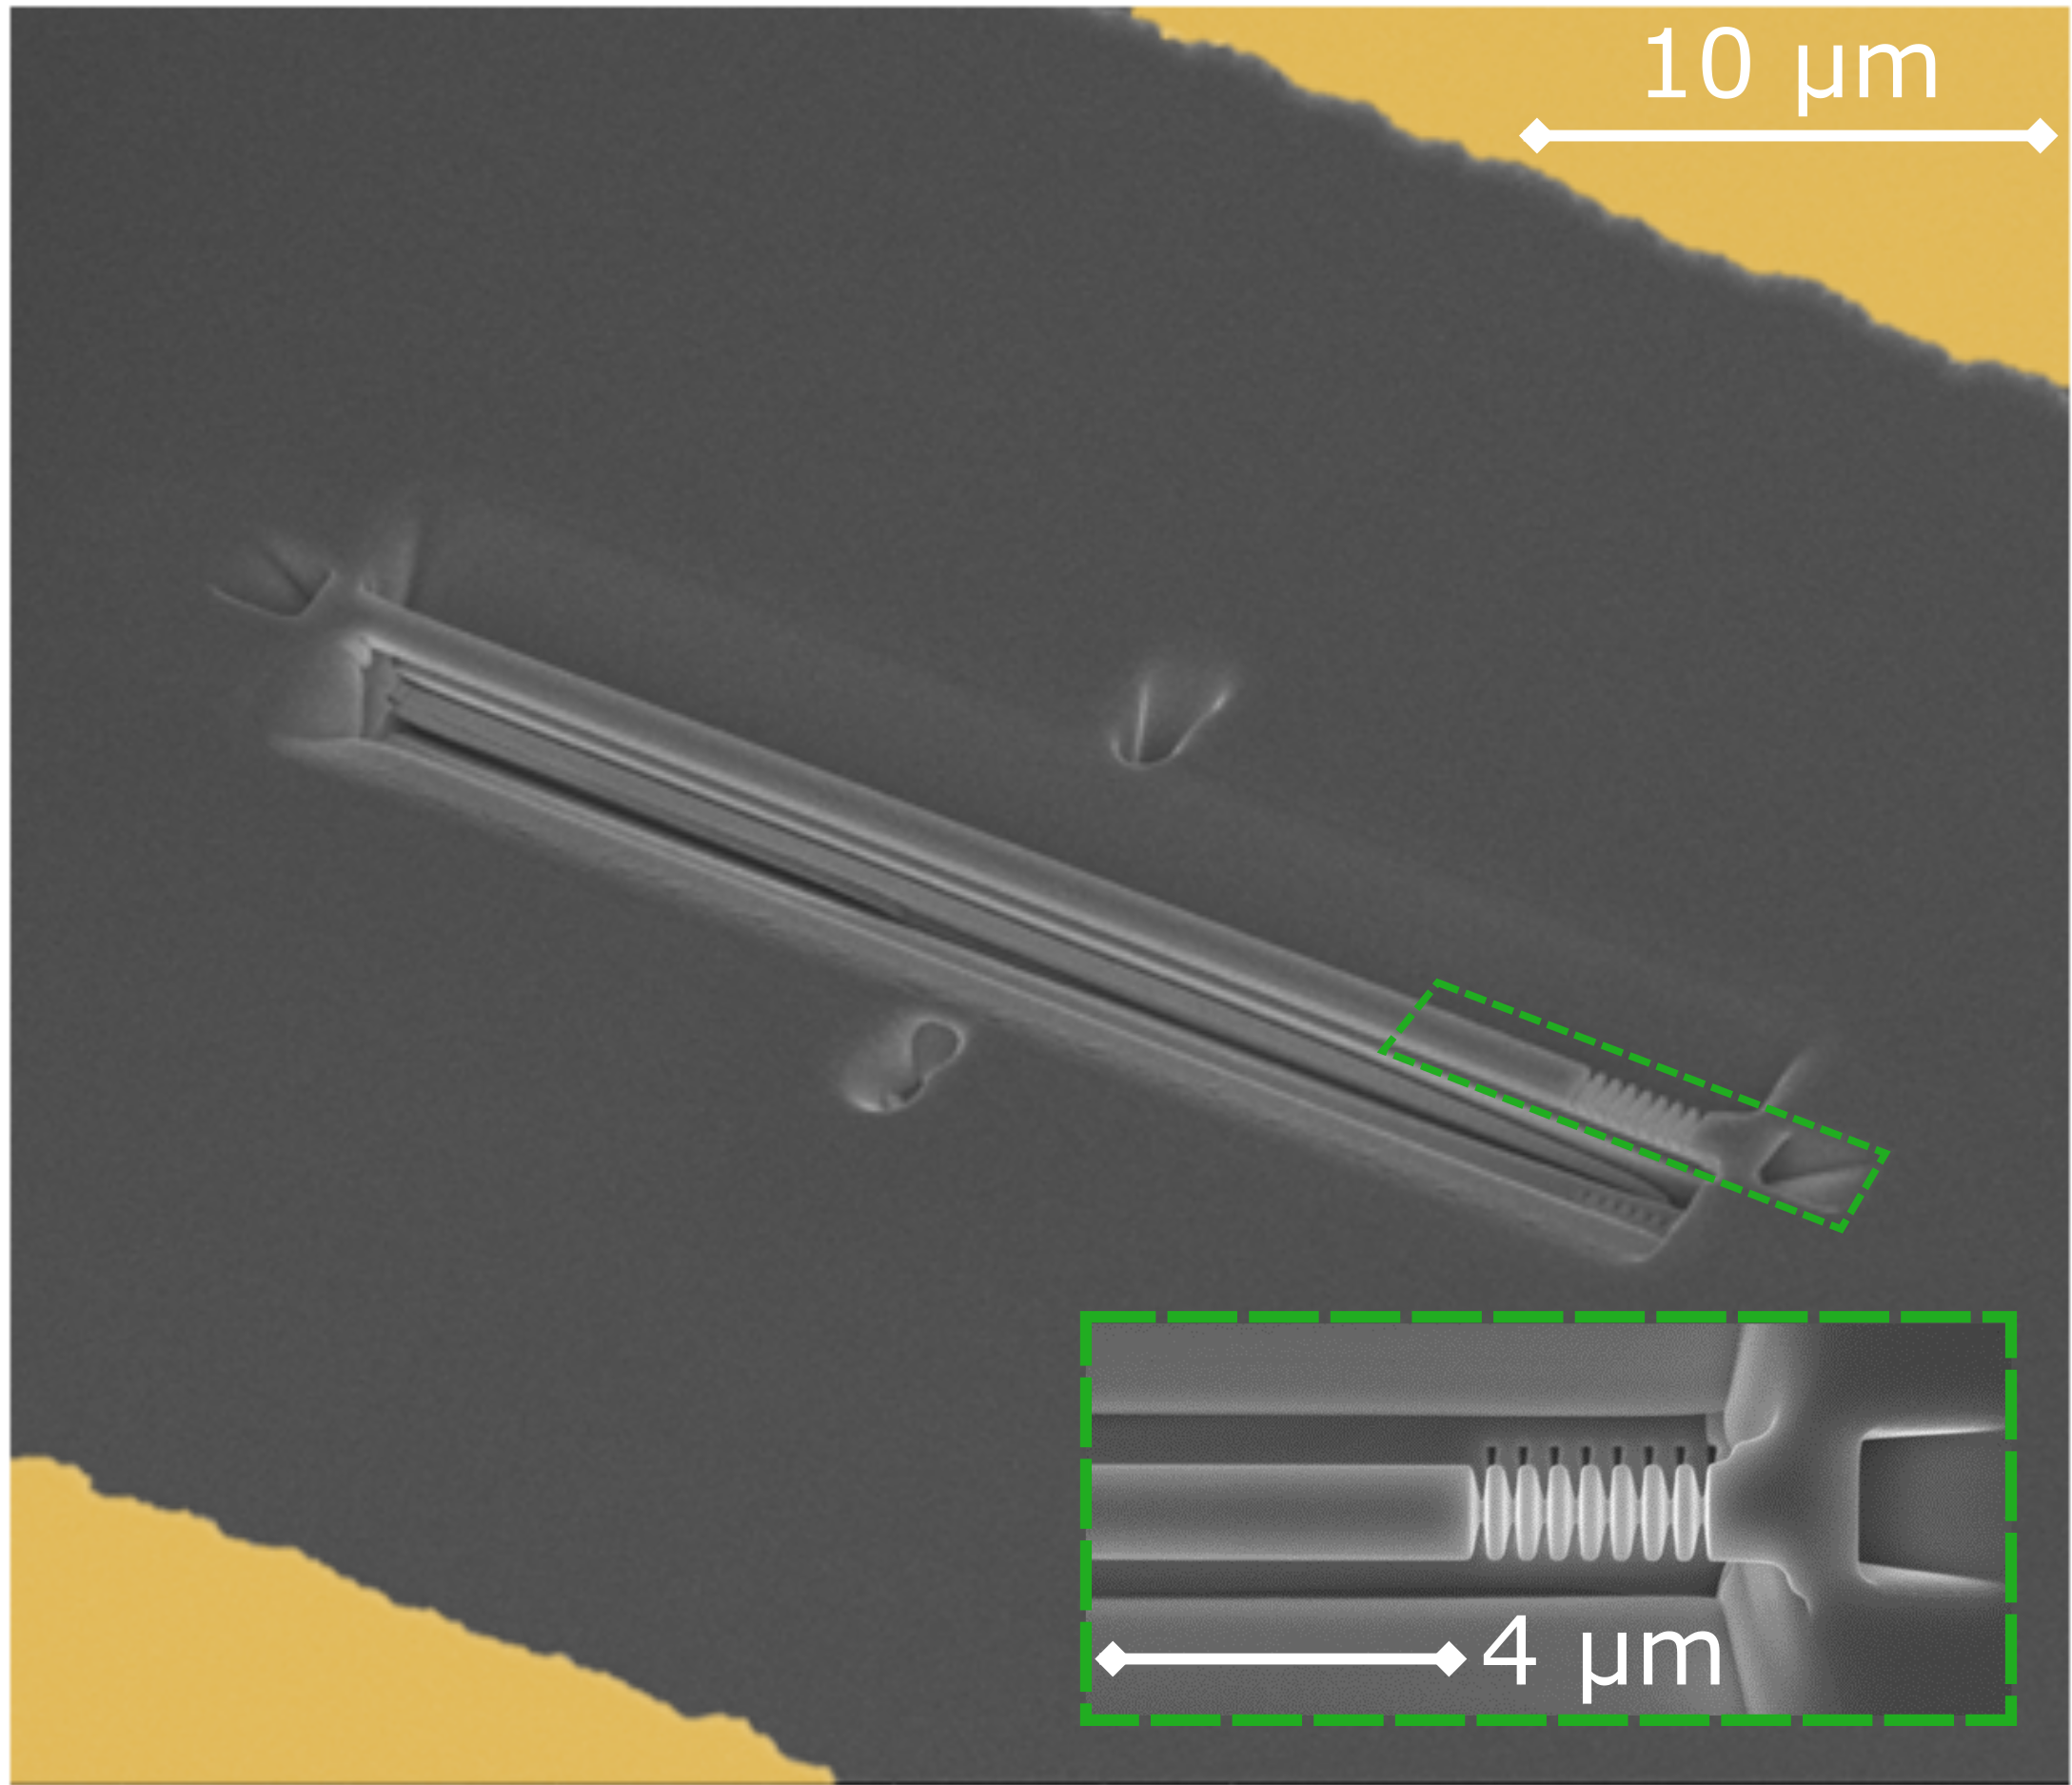
\includegraphics[height=55mm]{4lt-device}
\end{subfigure}
\begin{subfigure}{0.55\textwidth}
    \centering
    \includetikzpicture{four-level-diagram.tikz}
\end{subfigure}
\caption{\label{fig:4lt_device} \textbf{Left} The transduction device in Reference \cite{bartholomew_chip_2020}, consisting of a suspended optical waveguide constructed of \textsuperscript{171}Yb\textsuperscript{3+}:YVO\textsubscript{4}, terminating at a Bragg reflector so that signals enter and exit at the same end. Image credit: Reference \cite{bartholomew_chip_2020}. \textbf{Right} The four-level system in \textsuperscript{171}Yb\textsuperscript{3+}:YVO\textsubscript{4} used, annotated with transition frequencies at $B_z = \qty{2.09}{\milli\tesla}$ and with signal frequencies $\omega_\mu$, $\omega_p$, and $\omega_o$ of the transduction experiments. Shown in grey are the unused levels of the electronic quadruplets.}
\end{figure}

\begin{figure}[h!]
\centering
\includegraphics{4lt-example-scan}
\caption{\label{fig:four_level_transduction_experimental_data} Experimental transduction signals measured by sweeping $\omega_p$ and $\omega_\mu$. Left shows data captured using a weak optical pump in which the transduction signal consists of simple bright spots near the atomic transition frequencies (One for $\omega_p = \omega_{13}$ and one for $\omega_p = \omega_{23}$). Right shows data captured with a strong optical pump, which exhibits nontrivial structure with thin curve-like features. Data credit: Bartholomew et.\ al.\ (unpublished).}
\end{figure}

In constructing a model of four-level transduction. I aim to simulate the experiments described in Bartholomew et.\ al.\ 2020\cite{bartholomew_chip_2020}. This work used an on-chip device (Figure \ref{fig:4lt_device}) consisting of an optical waveguide constructed of \textsuperscript{171}Yb\textsuperscript{3+}:YVO\textsubscript{4} (yttrium orthovanadate doped with ytterbium) crystal, inside a microwave transmission line. For transduction experiments, the device is placed inside a dilution fridge and cooled to $\approx\qty{1}{\kelvin}$.

\textsuperscript{171}Yb\textsuperscript{3+}, the active species in transduction, has a nuclear spin $I=1/2$ and electron spin $S=1/2$. The energy levels of \textsuperscript{171}Yb\textsuperscript{3+} form electronic quadruplets that are non-degenerate (Zeeman-split) in the presence of an external magnetic field. The four levels relevant to the model are the upper two levels of the $^2F_{7/2}$ quadruplet ($\ket{1}$ and $\ket{2}$) and the lower two levels of the $^2F_{5/2}$ quadruplet ($\ket{3}$ and $\ket{4}$), which are separated by microwave transitions within a quadruplet and by near-infrared optical transitions between the quadruplets.

Transduction experiments in Reference \cite{bartholomew_chip_2020} consisted of an optical pump at $\omega_p$ that was swept between and around the $\omega_{13}$ and $\omega_{23}$ transition frequencies and a continuous microwave drive at $\omega_\mu$ that was swept around the $\omega_{34}$ transition frequencies, producing an optical output signal at $\omega_o = \omega_p + \omega_\mu$ through the $\ket{4}\to\ket{1}$ and $\ket{4}\to\ket{2}$ relaxations that is measured and recorded. Examples of these recorded transduction signal strengths are shown in Figure \ref{fig:four_level_transduction_experimental_data}.

This experimental data is used (in Section \ref{sec:4lt_results}) to benchmark the model, specifically a dataset that overlaps with the data published in Reference \cite{bartholomew_chip_2020}, but that also includes some unpublished data\footnote{Given to me by my supervisor who is the lead author of Reference \cite{bartholomew_chip_2020}}. This dataset consists of frequency scans for optical pump powers ranging from $\qty{-40}{\dBm}$ to $\qty{-4}{\dBm}$ inclusive. Published in Reference \cite{bartholomew_chip_2020} are experimental data in a weak optical pump regime in which the transduction signal simply consists of two spots around the two optical transition frequencies, which can be modelled as two separate three-level V-systems that do not significantly interact with each other. However, the unpublished data is in a strong optical pump regime in which the transduction signal contains features that stretch between both optical transitions. Reproducing these features was a goal of my modelling, and this requires a full four-level model.

\section{Driven Atom Hamiltonian}
The effect of the optical pump is represented by Rabi frequencies $\Omega_{13}$ and $\Omega_{23}$ on those respective transitions, because both are driven by the one pump. $\Omega_\mu$ is the Rabi frequency of the microwave drive on the $\ket{3}\to\ket{4}$ transition. Additionally, I include Rabi frequencies $\Omega_{14}$ and $\Omega_{24}$ to represent re-absorption of the emitted light by the atoms, possibly due to some back-reflection or weak cavity-like behaviour in the waveguide. Alternatively, these terms could be used in future modelling work for four-level atoms in cavities. Putting these together using blocks of Equation \ref{eq:two_level_time_dependent_rabi_hamiltonian}, the driven atom Hamiltonian in a static frame is
\begin{equation}
    \hat{H}_\text{static}(\omega'_{12}, \omega'_{13}, \omega'_{14}) =
    \begin{bmatrix}
        0 & 0 & \Omega_{13}^* e^{i\omega_p t} & \Omega_{14}^* e^{i\omega_o t}\\
        0 & \omega'_{12} & \Omega_{23}^* e^{i\omega_p t} & \Omega_{24}^* e^{i\omega_o t}\\
        \Omega_{13} e^{-i\omega_p t} & \Omega_{23} e^{-i\omega_p t} & \omega'_{13} & \Omega_\mu^* e^{i\omega_\mu t}\\
        \Omega_{14} e^{-i\omega_o t} & \Omega_{24} e^{-i\omega_o t} & \Omega_\mu e^{-i\omega_\mu t} & \omega'_{14}
    \end{bmatrix}
\end{equation}
where $\omega'_{ij} = \omega_{ij} - \delta_{ij}$ is, as in Subsection \ref{subs:steady_states}, the $\ket{i}\to\ket{j}$ transition frequency of the atom, which is different for each atom because of inhomogeneous broadening. A unitary transformation to a frame co-rotating with the signals gives a time-independent Hamiltonian
\begin{equation}
    \hat{H}(\delta_{12}, \delta'_p, \delta'_\mu) =
    \begin{bmatrix}
        0 & 0 & \Omega_{13}^* & \Omega_{14}^*\\
        0 & \omega'_{12} & \Omega_{23}^* & \Omega_{24}^*\\
        \Omega_{13} & \Omega_{23} & \delta'_p & \Omega_\mu^*\\
        \Omega_{14} & \Omega_{24} & \Omega_\mu & \delta'_p + \delta'_\mu
    \end{bmatrix}
\end{equation}
which is expressed in terms of detuning variables
\begin{align}
    \delta'_p &= \omega'_{13} - \omega_p = \delta_p - \delta_{13}\\
    \delta'_\mu &= \omega'_{34} - \omega_\mu = \delta_\mu - \delta_{34}.
\end{align}
The Master equation for the atoms is then
\begin{equation}
    \frac{d\hat{\rho}}{dt} =: \mathcal{L}(\delta_{12}, \delta'_p, \delta'_\mu)\hat{\rho} = -i[\hat{H}(\delta_{12}, \delta'_p, \delta'_\mu), \hat{\rho}] + \mathcal{L}_\text{dec}(\delta_{12}, \delta_{34})\hat{\rho}
\end{equation}
where the decoherence operator
\begin{equation}
\begin{split}
    \mathcal{L}_{\text{dec}}\hat{\rho} &= \mathcal{L}_{12}\hat{\rho} + \mathcal{L}_{13}\hat{\rho} + \mathcal{L}_{14}\hat{\rho} + \mathcal{L}_{23}\hat{\rho} + \mathcal{L}_{24}\hat{\rho} + \mathcal{L}_{2d}\hat{\rho} + \mathcal{L}_{3d}\hat{\rho} + \mathcal{L}_{4d}\hat{\rho}\\
    \mathcal{L}_{ij}\hat{\rho} &=
    \begin{cases}
        \begin{split}
            &\frac{\gamma_{ij}(n'_{ij}+1)}{2} \left(2\hat{\sigma}_{ij}\hat{\rho}\hat{\sigma}_{ji} - \hat{\rho}\hat{\sigma}_{jj} - \hat{\sigma}_{jj}\hat{\rho}\right)\\
            &+ \frac{\gamma_{ij}n'_{ij}}{2} \left(2\hat{\sigma}_{ji}\hat{\rho}\hat{\sigma}_{ij} - \hat{\rho}\hat{\sigma}_{ii} - \hat{\sigma}_{ii}\hat{\rho}\right)
        \end{split}
        & \text{$i=1,j=2$ or $i=3,j=4$}\\
        \frac{\gamma_{ij}}{2} \left(2\hat{\sigma}_{ij}\hat{\rho}\hat{\sigma}_{ji} - \hat{\rho}\hat{\sigma}_{j} - \hat{\sigma}_{jj}\hat{\rho}\right) & \text{otherwise}
    \end{cases}\\
    \mathcal{L}_{id}\hat{\rho} &= \frac{\gamma_{id}}{2} \left(2\hat{\sigma}_{ii}\hat{\rho}\hat{\sigma}_{ii} - \hat{\rho}\hat{\sigma}_{ii} - \hat{\sigma}_{ii}\hat{\rho}\right)
\end{split}
\end{equation}
is analogous to that of Equation \ref{eq:three_level_atom_loss_operator}, and depends on the microwave transition shifts via the thermal excitation counts of the microwave transition frequencies $n'_{12}$ and $n'_{34}$. The steady-state density matrix $\hat{\rho}_{SS}(\delta_{12}, \delta'_p, \delta'_\mu)$ can then be found by solving the linear system of the Master equation. In practice, I do this via the real version of the Master equation, as in Equation \ref{eq:real_master_equation}, because an $\mathbb{R}^{4\times 4}$ system of equations is faster to solve than a $\mathbb{C}^{4\times 4}$ system.

\section{Atomic Output}
Adapting from Equation \ref{eq:input_output_theory_output}, the input-output relation for a transition $\ket{i}\leftrightarrow\ket{j}$ of some atom is, up to some phase convention,
\begin{equation}
    \hat{a}_{\text{out},ij} = -\hat{a}_{\text{in},ij} + \sqrt{\gamma_{ij,c}} \hat{\sigma}_{ij}
\end{equation}
where $\gamma_{ij,c} \leq \gamma_{ij}$ is the relaxation rate of the atomic transition through coupling to the waveguide. To form a semiclassical approximation, I replace $\hat{a}_{\text{out},ij} \to \alpha_{\text{out},ij}$, as well as $\hat{a}_{\text{in},ij} \to \alpha_{\text{in},ij} = 0$ because the expectation value of the input is already captured by the Rabi frequencies on the atom Hamiltonian, and $\hat{\sigma}_{ij} \to \rho_{ji,SS}$ where I take the steady state, obtaining
\begin{equation}
    \alpha_{\text{out},ij}(\delta_{12}, \delta'_p, \delta'_\mu) = \sqrt{\gamma_{ij,c}} \rho_{SS,ji}.
\end{equation}
The output power from a given transition, then, is
\begin{equation}
    P_{\text{atom},ij}(\delta_{12}, \delta'_p, \delta'_\mu) = \hbar\omega_o \abs{\alpha_{\text{out},ij}}^2 = \hbar\omega_o \gamma_{ij,c}\abs{\rho_{SS,ji}}^2.
\end{equation}
Recall that there are two transitions producing output in this system, $\ket{1}\leftrightarrow\ket{4}$ and $\ket{2}\leftrightarrow\ket{4}$. The output power from each transition cannot simply be summed to obtain the total atomic output power, because each transition's emission may have different phases, and so they may interfere with each other. Specifically, because this model assumes that the light-matter interactions are through the dipole mechanism, the output has a phase related to that of the matrix element
\begin{equation}
    d_{ij} = \bra{i}\hat{d}_\parallel\ket{j}
\end{equation}
of the component of the dipole moment operator parallel to the emission polarisation. To capture this, I re-express the atomic relaxation rates in terms of complex numbers $C_{ij}$ for which
\begin{align}
    \abs{C_{ij}}^2 &= \gamma_{ij,c} \label{eq:C_ij_magnitude}\\
    \arg C_{ij} &= \arg d_{ij}. \label{eq:C_ij_phase}
\end{align}
Thus, the total atomic output power is
\begin{align}
    P_\text{atom}(\delta_{12}, \delta'_p, \delta'_\mu) &= \hbar\omega_o \abs{C_{14}\rho_{SS,41} + C_{24}\rho_{SS,42}}^2 =: \hbar\omega_o \Gamma_\text{atom}\\
    \Gamma_\text{atom}(\delta_{12}, \delta'_p, \delta'_\mu) &= \abs{C_{14}\rho_{SS,41} + C_{24}\rho_{SS,42}}^2
\end{align}
where $\Gamma_\text{atom}$ is the photon emission rate from the atom.

\section{Ensemble Output}
The total power $P(\delta_p, \delta_\mu)$ from the ensemble can be found as an integral of the single atom power $P_\text{atom}(\delta_{12}, \delta'_p, \delta'_\mu)$ over the inhomogeneous distribution
\begin{align}
    P(\delta_p, \delta_\mu) &= N \iiint p(\delta_{12}, \delta_{13}, \delta_{34}) P_\text{atom}(\delta_{12}, \delta_p-\delta_{13}, \delta_\mu-\delta_{34})\:d\delta_{12}d\delta_{13}d\delta_{34} \label{eq:four_level_total_power_no_approximation}\\
    &= \hbar\omega_oN \iiint p(\delta_{12}, \delta_{13}, \delta_{34}) \Gamma_\text{atom}(\delta_{12}, \delta_p-\delta_{13}, \delta_\mu-\delta_{34})\:d\delta_{12}d\delta_{13}d\delta_{34}
\end{align}
where $p(\delta_{12}, \delta_{13}, \delta_{34})$ is the PDF of the inhomogeneous distribution. I then make the approximation that the inhomogeneous shifts are much smaller than the transition frequencies $\abs{\delta_{ij}} \ll \omega_{ij}$. $\Gamma_\text{atom}$ depends on $\delta_{12}$ only via the shifted transition frequency $\omega'_{12}$, and in this approximation $\omega'_{12} \approx \omega_{12}$, and so $\delta_{12}$ can be ignored. This is not true of the other shifts $\delta_{13}$ and $\delta_{34}$ because $\Gamma_\text{atom}$ depends on them directly. In this approximation, then,
\begin{align}
    P(\delta_p, \delta_\mu) &= \hbar\omega_{o}N \iint p(\delta_{13}, \delta_{34}) \Gamma_\text{atom}(\delta_p-\delta_{13}, \delta_\mu-\delta_{34})\:d\delta_{13}d\delta_{34} \label{eq:four_level_total_power_approximated}\\
    &= \hbar(\omega_{14}-\delta_p-\delta_\mu)N (p * \Gamma_\text{atom}) \label{eq:four_level_total_power_convolution}
\end{align}
where $p(\delta_{13}, \delta_{34}) = \int p(\delta_{12}, \delta_{13}, \delta_{34})\:d\delta_{12}$ is a marginal PDF, and $\omega_o$ has been re-expressed explicitly in terms of the detuning variables. Thus, numerically evaluating a grid of $P(\delta_p, \delta_\mu)$ is a matter of first evaluating a grid of $\Gamma_\text{atom}(\delta'_p, \delta'_\mu)$ and then convolving it with a grid of $p(\delta_{13}, \delta_{34})$, which is much cheaper computationally than evaluating the integral in Equation \ref{eq:four_level_total_power_no_approximation} (or even Equation \ref{eq:four_level_total_power_approximated}) using numerical quadrature because convolutions can be evaluated using Fast Fourier Transform. Furthermore, in the experiments that I am modelling, $\abs{\delta_p}, \abs{\delta_\mu} \ll \omega_{14}$, and so the expression for $\omega_o$ in Equation \ref{eq:four_level_total_power_convolution} simplifies to
\begin{equation}
    P = \hbar\omega_{14}N (p * \Gamma_\text{atom}). \label{eq:four_level_total_power_convolution_approximate}
\end{equation}

\section{Numerical Methods}
As can be seen in Figure \ref{fig:four_level_transduction_experimental_data}, there are thin curve-like features in the transduction signal. When evaluating a grid of $\Gamma_\text{atom}$, these curve features may be subject to grid \textit{aliasing}, in which the relative alignment of the features with the grid points result in unphysical structure in the resulting grid of $\Gamma_\text{atom}$ values, which is then blown up in $P$ by convolution. In this section, I describe the methods I use to implement the model in a manner that is robust to grid aliasing while being computationally cheaper than simply using a finer grid.

\subsection{Grid Aliasing}
A mathematical description of grid aliasing is as follows. Letting $\Delta_{13}$ and $\Delta_{34}$ be the grid spacing of the discretised convolution kernel $p$, the discretised convolution in Equation \ref{eq:four_level_total_power_convolution_approximate} is
\begin{align}
    P(\delta_p, \delta_\mu) &\approx \hbar\omega_{14}N \sum_{(i,j)\in\mathbb{Z}^2} p(i\Delta_{13}, j\Delta_{34}) \Gamma_\text{atom}(\delta_p-i\Delta_{13}, \delta_\mu-j\Delta{34})\\
    &= \iint \underbrace{p(\delta_{13}, \delta_{34}) \Sh_{\Delta_{13}}(\delta_{13}) \Sh_{\Delta_{34}}(\delta_{34})}_\text{convolution kernel} \Gamma_\text{atom}(\delta_p-\delta_{13}, \delta_\mu-\delta_{34})\:d\delta_{13}d\delta_{34}
\end{align}
where $\Sh_T(x)$ is a Dirac comb of period $T$. This means that discretising the convolution in Equation \ref{eq:four_level_total_power_convolution_approximate} is equivalent to discretising the kernel into a weighted Dirac comb. Convolving with this kernel, unlike the original kernel, does not smooth out curve features, but merely displaces them, which is precisely the aliasing mentioned earlier. However, if our grid of $\Gamma_\text{atom}$ contained the integral within the neighbourhood of a grid point instead of just the value at the grid point itself, the discretised convolution would be
\begin{align}
    P(\delta_p, \delta_\mu) &\approx \hbar\omega_{14}N \sum_{(i,j)\in\mathbb{Z}^2} p(i\Delta_{13}, j\Delta_{34}) \int_{i-1/2}^{i+1/2} \int_{j-1/2}^{j+1/2} \Gamma_\text{atom}(\delta_p-i'\Delta_{13}, \delta_\mu-j'\Delta{34})\:di'dj'\\
    &= \iint \underbrace{p([i]\Delta_{13}, [j]\Delta_{34})}_\text{convolution kernel} \Gamma_\text{atom}(\delta_p-i\Delta_{13}, \delta_\mu-j\Delta_{34})\:didj
\end{align}
where $[x]$ is the rounding of $x$ to the nearest integer. This convolution kernel is a step function, which is both closer to the original kernel than a weighted Dirac comb, and smooths out curve features because it is finite everywhere. Evaluating this integral within a neighbourhood for every grid point, however, is equivalent to simply evaluating the discrete convolution with a finer grid, which is the trivial way to deal with aliasing. Instead, my approach is to determine which neighbourhoods contain curve features, and replace only those grid points' values with integrals.

\subsection{Feature Finding}
\begin{figure}[h]
\centering
\includetikzpicture{feature-finding.tikz}
\caption{\label{fig:feature_finding} An illustration of feature finding. The grid squares are neighbourhoods around grid points, and the thick curves represent the features we want to find. The intersections of the feature curves with the neighbourhood edges are shown by circles, and the neighbourhoods containing these features are highlighted grey.}
\end{figure}

To find which neighbourhoods contain curve features, it suffices to simply identify the points of intersection of these features with the edges of neighbourhoods, so that any neighbourhood lying on such an edge contains a curve feature\footnote{Alternatively, curve features could be closed loops contained entirely within that single neighbourhood. I have not observed closed loop features in practice, and even if they do exist, a grid that is coarse enough to contain an entire such loop within a single point's neighbourhood is too coarse to be very useful.}. This is illustrated in Figure \ref{fig:feature_finding}. For an $n\times m$ grid, this process allows all $nm$ neighbourhoods of grid points to be tested for feature presence by testing only the $(n+1)(m+1)$ lines that form edges between them.

As mentioned in Subsection \ref{ssubs:barnett_longdell_numerical_methods}, Reference \cite{barnett_longdell_2020} identified that curve features occur where the discriminant of the characteristic polynomial of the atom Hamiltonian
\begin{equation}
    \Delta(\delta'_p, \delta'_\mu) = \text{Disc}_\lambda\left(\det\left(\hat{H}(\delta'_p, \delta'_\mu)-\lambda\hat{\mathds{1}}\right)\right)
\end{equation}
has its roots. Because the Hamiltonian is Hermitian and therefore its characteristic polynomial has exclusively real roots, this discriminant is uniformly non-negative. This means all roots of the discriminant are `partial' (single-variable) local minima, and it is more numerically stable to identify partial local minima via roots of the discriminant's partial derivative than to directly find roots of the discriminant itself\cite{barnett_msc}. Reference \cite{barnett_longdell_2020} used generic numerical root-finding, but I instead use polynomial-specific root-finding that uses the polynomial coefficients of $\Delta(\delta'_p, \delta'_\mu)$ and its partial derivatives. This has the advantage of finding all roots rather than just one.

\begin{figure}[h!]
\centering
\includegraphics{4lt-pixel-intersections.png}
\caption{\label{fig:pixel_intersections} $\Gamma_\text{atom}$ grids with curve feature intersections identified by along-edge partial local minima (white circles) and across-edge partial local minima (black circles). Left has the same domain as Figure \ref{fig:four_level_transduction_experimental_data} and shows aliasing artefacts along curve features, and right is a close-up around a curve feature, showing duplicate identification and misalignment from the feature's centre.}
\end{figure}

The procedure is as follows.
\begin{enumerate}
    \item Precompute the bivariate polynomial coefficients of $\Delta(\delta'_p, \delta'_\mu)$, $\frac{\partial\Delta}{\partial\delta'_p}(\delta'_p, \delta'_\mu)$, $\frac{\partial^2\Delta}{{\partial\delta'_p}^2}(\delta'_p, \delta'_\mu)$, $\frac{\partial\Delta}{\partial\delta'_\mu}(\delta'_p, \delta'_\mu)$, and $\frac{\partial^2\Delta}{{\partial\delta'_\mu}^2}(\delta'_p, \delta'_\mu)$, because only the detuning variables change over this process.
    \item To find all the intersections along some $\delta'_p$ edge (constant $\delta'_\mu$), evaluate the univariate polynomial coefficients of $\frac{\partial\Delta}{\partial\delta'_p}(\delta'_p)$ for the edge's $\delta'_\mu$, and perform root-finding with them to find all critical points of $\Delta(\delta'_p)$.
    \item Evaluate $\Delta$ at each critical point. Critical points whose values of $\Delta$ are smaller than those of their immediately adjacent critical points are local minima and are therefore taken to be curve feature intersections.
    \item Evaluate the polynomial coefficients of $\frac{\partial\Delta}{\partial\delta'_\mu}(\delta'_p)$ and use them to find critical points of $\Delta(\delta'_\mu)$.
    \item Evaluate the polynomial coefficients of $\frac{\partial^2\Delta}{{\partial\delta'_\mu}^2}(\delta'_p)$ and use them to perform the second derivative test $\frac{\partial^2\Delta}{{\partial\delta'_\mu}^2} \geq 0$ for each critical point of $\Delta(\delta'_\mu)$ to identify local minima.
\end{enumerate}
This process is repeated for each $\delta'_p$ edge, and then vice-versa ($\delta'_p$ and $\delta'_\mu$ swapped) for all $\delta'_\mu$ edges (constant $\delta'_p$).

For each of the two edge directions, both partial local minima along the edge and perpendicular to the edge are identified by this procedure. However, there is an asymmetry between these in that the former use direct comparisons between critical points and the latter use a second derivative test; the latter is to avoid having to evaluate extra $\Delta$ values outside the edge being tested. Furthermore, the second derivative test is done inclusive of exact equality in order to err on the side of false positives rather than false negatives.

\begin{figure}[h!]
\centering
\input{trench-duplication.pgf}
\caption{\label{fig:trench_duplication} Around a curve feature, $\Delta$ often takes the shape of a `trench' which is non-constant at its bottom. When scanning the gradient (arrows) of $\Delta$ in such a region, the gradient flips around on either side, but it is not zero at any point, and so it rotates through the parallel and perpendicular (orange arrows), resulting in this curve feature being found twice.}
\end{figure}

As is shown by Figure \ref{fig:pixel_intersections}, this procedure successfully identifies curve features that produce aliasing artefacts. Additionally, there are curve feature intersections that are found only by the across-edge test, and not the along-edge test, and so this test is necessary to find all grid point neighbourhoods containing curve features. Checking both parallel and perpendicular partial local minima, however, has the side effect of causing many curve features to be identified twice, but this has no effect beyond slightly increasing computational cost. The reasons for this are explained in Figure \ref{fig:trench_duplication}. Additionally, these partial local minima are often very slightly misaligned from the actual curve features, by an amount that is much smaller than most useful grid spacings, and that therefore does not have any significant effect on the final results of this process.

\begin{figure}[h!]
\centering
\includetikzpicture{neighbourhood-integration.tikz}
\caption{\label{fig:neighbourhood_integration} The integration within a single grid point's neighbourhood. The curve feature has an axis-aligned bounding box (dashed) computed from its edge intersections (filled circles) that is wider than it is tall proportional to the neighbourhood's dimensions, and so the outer integral is horizontal and the inner integral (which is represented by the vertical arrows) is vertical. The inner integral's domain is split at curve feature intersections (and surrounding points, which are not shown here).}
\end{figure}

\subsection{Neighbourhood Integration}
Once the points whose neighbourhoods contain curve features are identified, the integral within the neighbourhood must be evaluated using some numerical quadrature scheme. To do this, I use the discriminant once again to perform importance sampling along an inner integral, using Gauss-Lobatto quadrature, as in Reference \cite{barnett_longdell_2020}. For each intersection point, the inner integral's domain is split at intersections with curve features, as well as at addition points surrounding the intersections, with each interval between splits evaluated using a separate instance of Gauss-Lobatto quadrature. If the inner integral is along $\delta'_p$, then for each curve intersection ${\delta'_p}^{(*)}$, the split points are ${\delta'_p}^{(*)}$ itself, ${\delta'_p}^{(*)} \pm \gamma_{ph}$, ${\delta'_p}^{(*)} \pm 3\gamma_{ph}$, and ${\delta'_p}^{(*)} \pm 10\gamma_{ph}$, where $\gamma_{ph} = \gamma_{3d}$ is used as an estimate of the homogeneous linewidth and therefore the thickness of the curve feature. If the inner integral is along $\delta'_\mu$, the splits points from each intersection ${\delta'_\mu}^{(*)}$ are the intersection itself as well as ${\delta'_\mu}^{(*)} \pm \gamma_{\mu h}$, ${\delta'_\mu}^{(*)} \pm 3\gamma_{\mu h}$, and ${\delta'_\mu}^{(*)} \pm 10\gamma_{\mu h}$, where $\gamma_{\mu h} = \gamma_{3d} + \gamma_{4d}$. Split points outside the bounds of the integral (the neighbourhood edges) are excluded.

Reference \cite{barnett_longdell_2020} chose the inner and outer integral axes arbitrarily, but the outer integral would ideally be as close to parallel to the curve feature as possible, because that minimises the distance along the curve between sample points. To handle this, I re-use the curve intersection data computed in the previous step to find an axis-aligned bounding box for the curve feature inside the neighbourhood, and let the outer integral axis be the axis along which this bounding box takes up the largest fraction of the neighbourhood's size (Figure \ref{fig:neighbourhood_integration}).

\section{\label{sec:4lt_parameters}Experimental Parameters for Model}
To summarise, this model requires as input the following parameters:
\begin{itemize}
    \item Microwave transition frequencies $\omega_{12}$ and $\omega_{34}$
    \item Rabi frequencies $\Omega_{13}$, $\Omega_{23}$, $\Omega_{14}$, $\Omega_{24}$, and $\Omega_\mu$
    \item Microwave transition relaxation lifetimes $\tau_{12}$ and $\tau_{34}$ and operating temperature $T$
    \item Optical transition relaxation rates $\gamma_{13}$, $\gamma_{23}$, $\gamma_{14}$, and $\gamma_{24}$
    \item Optical output waveguide couplings $C_{14}$ and $C_{24}$
    \item Inhomogeneous PDF $p(\delta_{13}, \delta_{34})$
    \item Atom count N and optical transition frequency $\omega_{14}$.
\end{itemize}
$N$ merely scales the output signal power uniformly, and therefore does not need much precision, and can be found through trial and error. Reference \cite{bartholomew_chip_2020} quotes an estimate for the operating temperature of $T \approx \qty{1}{\kelvin}$, and a microwave Rabi frequency $\Omega_\mu = 2\pi \times \qty{1}{\mega\hertz}$.

\subsection{Inhomogeneous Broadening}
Reference \cite{bartholomew_chip_2020} specifies the inhomogeneous distribution as Gaussian with standard deviations $\Gamma_{\text{ih},o} \approx \qty{200}{\mega\hertz}$ for optical transitions and $\Gamma_{\text{ih},\mu} \approx \qty{130}{\kilo\hertz}$ for microwave transitions, with a correlation slope of $\num{-120}$ ($\text{optical}/\text{microwave}$) between them. Using the formula
\begin{equation}
    \text{slope} := \frac{\Delta y}{\Delta x} = \frac{\sigma_{xy}}{\sigma_x^2}
\end{equation}
gives a covariance of $\qty{-2.028}{\mega\hertz\squared}$, and so the inhomogeneous PDF is that of the bivariate normal distribution
\begin{align}
    p\left(\vec{\delta} =
    \begin{bmatrix}
        \delta_{13}\\
        \delta_{34}
    \end{bmatrix}\right)
    &=
    \frac{1}{\sqrt{2\pi\det\Sigma}} \exp\left(-\frac{1}{2}\vec{\delta}^T\Sigma^{-1}\vec{\delta}\right)\\
    \Sigma &=
    \begin{bmatrix}
        (\qty{200}{\mega\hertz})^2 & \qty{-2.028}{\mega\hertz\squared}\\
        \qty{-2.028}{\mega\hertz\squared} & (\qty{130}{\kilo\hertz})^2
    \end{bmatrix}.
\end{align}

\subsection{Spin Hamiltonian}
To find the remaining parameters, I make use of the spin Hamiltonians\cite{kindem_characterization_2018} of the two electronic quadruplets in this system
\begin{equation}
    \hat{H}_{g,e} = \mu_B\vec{B}^Tg_{g,e}\vhat{S} + \vhat{I}^TA_{g,e}\vhat{S} \label{eq:spin_hamiltonian_compact}
\end{equation}
where subscripts $g$ and $e$ are indices indicating the ground ($^2F_{7/2}$) and excited ($^2F_{5/2}$) multiplets respectively, $g_{g,e}$ are Zeeman interaction tensors, and $A_{g,e}$ are hyperfine interaction tensors. $\vec{B}$ is the external magnetic field, $\vhat{S} = [\hat{S}_x, \hat{S}_y, \hat{S}_z]^T$ is the electron spin operator and $\vhat{I} = [\hat{I}_x, \hat{I}_y, \hat{I}_z]^T$ is the nuclear spin operator. The symmetry of the crystal site occupied by ytterbium ions\footnote{In the usual crystallography notation, this is the $D_{2d}$ symmetry group} means that the $g_{g,e}$ and $A_{g,e}$ tensors have two eigenvalues, one unique (multiplicity $1$) and one non-unique (multiplicity $2$). Denoting the unique eigenvalues as $g_{\parallel g,e}$ and $A_{\parallel g,e}$ and the non-unique eigenvalues as $g_{\perp g,e}$ and $A_{\perp g,e}$, Equation \ref{eq:spin_hamiltonian_compact} expands into
\begin{equation}
    \hat{H}_{g,e} = \mu_B[g_{\perp g,e}(B_x\hat{S}_x + B_y\hat{S}_y) + g_{\parallel g,e}B_z\hat{S}_z] + A_{\perp g,e}(\hat{I}_x\hat{S_x} + \hat{I}_y\hat{S}_y) + A_{\parallel g,e}\hat{I}_z\hat{S}_z \label{eq:spin_hamiltonian_expanded}
\end{equation}
where it is assumed without generality that $z$ is the unique axis and $x$ and $y$ are the non-unique axes\footnote{In the usual crystallography notation, $c\parallel z$}. The magnetic field in the benchmarking dataset is $\vec{B} = [0, 0, \qty{2.09}{\milli\tesla}]^T$, of which the only nonzero component is $B_z$, but the other components are kept for later calculations regarding magnetic field noise. The interaction tensor elements are shown in Table \ref{tab:spin_hamiltonian_parameters}.

\begin{table}[h]
\centering
\begin{tabular}{c|c}
Parameter & Value\\
\hline
$g_{\perp g}$ & $\num{0.85}$\\
$g_{\parallel g}$ & $\num{-6.08}$\\
$g_{\perp e}$ & $\num{1.7}$\\
$g_{\parallel e}$ & $\num{2.51}$\\
$A_{\perp g}$ & $2\pi \times \qty{675}{\mega\hertz}$\\
$A_{\parallel g}$ & $2\pi \times \qty{-4.82}{\giga\hertz}$\\
$A_{\perp e}$ & $2\pi \times \qty{3.37}{\giga\hertz}$\\
$A_{\parallel e}$ & $2\pi \times \qty{4.86}{\giga\hertz}$\\
\end{tabular}
\caption{\label{tab:spin_hamiltonian_parameters} Interaction tensor elements of the spin Hamiltonian in Equation \ref{eq:spin_hamiltonian_expanded}. $g_{\perp g}$ and $g_{\parallel g}$ are from Reference \cite{ranon_1968}, and the remaining values are from from Reference \cite{kindem_characterization_2018}.}
\end{table}

\subsection{Transition Frequencies}
The eigenvectors of $\hat{H}_g$ are the four levels of the multiplet (Figure \ref{fig:4lt_device}), and so the transition frequencies within a multiplet are simply the difference of the corresponding eigenvalues, which gives us
\begin{align}
    \omega_{12} &= \bra{2}\hat{H}_g\ket{2} - \bra{1}\hat{H}_g\ket{1}\\
    \omega_{34} &= \bra{4}\hat{H}_e\ket{4} - \bra{3}\hat{H}_e\ket{3}
\end{align}
where $\hat{H}_{g,e}$ are evaluated with $B_z = \qty{2.09}{\milli\tesla}$. At zero magnetic field\cite{bartholomew_chip_2020}, $\omega_{13} = 2\pi \times \qty{304501.0}{\giga\hertz}$, and because this is only used to calculate the scale of the output energy (via $\omega_{14} = \omega_{12} + \omega_{23} + \omega_{34}$), this is a good enough approximation of the value at $B_z = \qty{2.09}{\milli\tesla}$.

\subsection{Dephasing Rates}
If we assume that magnetic field noise, which would be caused by the nuclear spin flips in the yttrium and vanadium of the host crystal, is the dominant source of dephasing in this system, then the dephasing rates are proportional to
\begin{equation}
    \gamma_{id} \propto \norm{\frac{d\omega_{1i}}{d\vec{B}}}^2.
\end{equation}
The transition frequency is
\begin{equation}
    \omega_{1i} = \bra{i}\hat{H}_{g,e}\ket{i} - \bra{1}\hat{H}_g\ket{1}
\end{equation}
where the index on the first $\hat{H}_{g,e}$ is $g$ if $i=2$ and $e$ if $i\in\{3,4\}$. Substituting Equation \ref{eq:spin_hamiltonian_expanded} and differentiating, we obtain
\begin{equation}
    \gamma_{id} \propto \norm{g_{g,e} \bra{i}\vhat{S}\ket{i} - g_g \bra{1}\vhat{S}\ket{1}}^2 \label{eq:spin_hamiltonian_dephasing}
\end{equation}
where the index on the first $g_{g,e}$ is the same index as the one on $\hat{H}_{g,e}$. In practice, $\hat{S}_z$ is the only nonzero component of $\vhat{S}$ when restricting these operators to the $(\ket{1}, \ket{2}, \ket{3}, \ket{4})$ basis, and so Equation \ref{eq:spin_hamiltonian_dephasing} becomes
\begin{equation}
    \gamma_{id} \propto \abs{g_{\parallel g,e} \bra{i}\hat{S}_z\ket{i} - g_{\parallel g} \bra{1}\hat{S}_z\ket{1}}^2. \label{eq:spin_hamiltonian_z_dephasing}
\end{equation}

\subsection{Dipole Moments}
The remaining parameters are proportional to dipole moment matrix elements. These include the atomic coupling depolarisation rates
\begin{equation}
    \gamma_{ij,c} \propto \vec{d}_{ij} = \norm{\bra{i}\vhat{d}\ket{j}}^2 \label{eq:depolarisation_proportionality}
\end{equation}
as well as, from Equation \ref{eq:rabi_frequency_dipole_moment},
\begin{equation}
    \Omega_{ij} \propto d_{\parallel ij} \label{eq:rabi_frequency_proportionality}
\end{equation}
where $d_{\parallel ij}$ is the component of $\vec{d}_{ij}$ parallel to the drive polarisation. In this system, both electric and magnetic dipoles are proportional to electron spin
\begin{equation}
    \vhat{d} \propto \vhat{S},
\end{equation}
and so the spin Hamiltonian can once again be used. First of all, Equation \ref{eq:rabi_frequency_proportionality} gives a ratio
\begin{equation}
    \frac{\Omega_{13}}{\Omega_{23}} = \frac{\bra{1}\hat{S}_z\ket{3}}{\bra{2}\hat{S}_z\ket{3}} \label{eq:optical_rabi_frequency_ratio}
\end{equation}
between the optical pump Rabi frequencies, where the fact that $\hat{S}_z$ is the only nonzero spin component has once again been used. The remaining optical Rabi frequencies are set to zero ($\Omega_{14}=0=\Omega_{24}$) because the transduction efficiencies in the benchmarking dataset are quite low ($<10^{-5}$). Second, from Reference \cite{kindem_characterization_2018}, $\gamma_{14}(\vec{B}=\vec{0}) = \qty{1.4}{\kilo\hertz}$ and $\gamma_{23}(\vec{B}=\vec{0}) = \qty{1.3}{\kilo\hertz}$, and optical transitions $\ket{1}\leftrightarrow\ket{3}$ and $\ket{2}\leftrightarrow\ket{4}$ are forbidden at zero magnetic field. In terms of the spin operators, these forbidden transitions are reflected by the fact that
\begin{align}
    \bra{1}\hat{S}_z(\vec{B}=\vec{0})\ket{4} &= -\bra{2}\hat{S}_z(\vec{B}=\vec{0})\ket{3} \neq 0\\
    \bra{1}\hat{S}_z(\vec{B}=\vec{0})\ket{3} &= \bra{2}\hat{S}_z(\vec{B}=\vec{0})\ket{4} = 0.
\end{align}
The fact that dipole-forbidden transitions have depolarisation rates much lower than dipole-permitted transitions shows that these optical depolarisations happen predominantly through dipole emission, and so I set $\gamma_{ij}=\gamma_{ij,c}$. At $B_z=\qty{2.09}{\milli\tesla}$, $\bra{1}\hat{S}_z\ket{3} = \bra{2}\hat{S}_z\ket{4}$ take on a small nonzero value, and $\bra{1}\hat{S}_z\ket{4} = -\bra{2}\hat{S}_z\ket{3}$ decrease in magnitude as the levels hybridise. Using Equation \ref{eq:depolarisation_proportionality},
\begin{equation}
\begin{split}
    \gamma_{14} &= \frac{\abs{\bra{1}\hat{S}_z\ket{4}}^2}{\abs{\bra{1}\hat{S}_z(\vec{B}=\vec{0})\ket{4}}^2} \gamma_{14}(\vec{B}=\vec{0})\\
    \gamma_{23} &= \frac{\abs{\bra{2}\hat{S}_z\ket{3}}^2}{\abs{\bra{2}\hat{S}_z(\vec{B}=\vec{0})\ket{3}}^2} \gamma_{23}(\vec{B}=\vec{0})\\
    \gamma_{13} &= \frac{\abs{\bra{1}\hat{S}_z\ket{3}}^2}{\abs{\bra{2}\hat{S}_z\ket{3}}^2} \gamma_{23}\\
    \gamma_{24} &= \frac{\abs{\bra{2}\hat{S}_z\ket{4}}^2}{\abs{\bra{1}\hat{S}_z\ket{4}}^2} \gamma_{23}\\
\end{split}
\label{eq:optical_relaxation_hybridisation}
\end{equation}
and $C_{14}$ and $C_{24}$ are set accordingly by Equations \ref{eq:C_ij_magnitude} and \ref{eq:C_ij_phase}. From Reference \cite{kindem_control_2020}, $\tau_{12}(\vec{B}=\vec{0}) = \qty{54}{\milli\second}$, and so
\begin{equation}
    \tau_{12} = \frac{\abs{\bra{1}\hat{S}_z(\vec{B}=\vec{0})\ket{2}}^2}{\abs{\bra{1}\hat{S}_z\ket{2}}^2} \tau_{12}(\vec{B}=\vec{0}). \label{eq:tau_12_hybridisation}
\end{equation}
In the absence of data on $\tau_{34}$, I set it to $\qty{10}{\milli\second}$, to match the order of magnitude of $\tau_{12}$.

\subsection{Optical Pump Calibration}
From Equation \ref{eq:rabi_frequency_dipole_moment}, $\Omega_{23} \propto \sqrt{P}$ where $P$ is the pump power. The equation for this proportionality, appropriately calibrated, is
\begin{equation}
    \Omega_{23} = \frac{\Omega_{23,\text{ref}}\sqrt{\eta}}{\sqrt{P_\text{ref}}} \sqrt{P}
\end{equation}
where $(\Omega_{23,\text{ref}}, P_\text{ref})$ is some known `reference' Rabi frequency-power pair for calibration, and $\eta$ is the efficiency with which power from the source makes it into the waveguide. Reference \cite{bartholomew_chip_2020} contains a frequency-power pair $(\Omega_{23,\text{ref}}=2\pi\times\qty{6}{\mega\hertz}, P_\text{ref}=\qty{2}{\micro\watt})$, and my supervisor provided data with which to calibrate the efficiency to $\eta=\num{0.055}$ (Appendix \ref{ap:4lt_power_calibration}). 

\section{\label{sec:4lt_results}Results}
\begin{figure}[h]
\centering
\includegraphics{4lt-model-scan}
\caption{\label{fig:4lt_model_scan} Power-frequency grids from the model when obeying the constraints found in Section \ref{sec:4lt_parameters} (left) and when disobeying those constraints (middle) as compared with the experimental data (right) shown in Figure \ref{fig:four_level_transduction_experimental_data}, with optical pump power $\qty{-4}{\dBm}$. All three plots have the same frequency and colour scales. A simple noise model is used in this comparison.}
\end{figure}

To evaluate the model, I computed power-frequency grids with frequency domain and input parameters corresponding to the experimental data. Because the model does not include the noise in the experimental apparatus, I add simulated noise to the computed power. This consists of random samples from the experimental frequency sweep with $\qty{-40}{\dBm}$ optical pump power, which contains no discernible transduction signal, only noise. A comparison of the resultant power-frequency grids with experimental data is shown in Figure \ref{fig:4lt_model_scan}.

After the analysis in Section \ref{sec:4lt_parameters}, the remaining free parameters are $N$ and $\gamma_{2d}$, as well as some leeway in adjusting $\Omega_{23}$ since the calibration parameters $\Omega_{23,\text{ref}}$ and $P_\text{ref}$ have only one significant figure of precision. I adjusted these free parameters to find a set of parameters that best replicated the experimental data, which resulted in $N=\num{1e14}$, $\gamma_{2d}=\qty{10}{\kilo\hertz}$, and an adjustment to the $\Omega_{23}$ calibration of $P_\text{ref}=\qty{1.7}{\micro\watt}$.

This showed only superficial qualitative agreement, and so I next adjusted the parameters while breaking the constraints identified in Section \ref{sec:4lt_parameters}, finding better agreement with $N=\num{1e10}$, $\tau_{12}(\vec{B}=\vec{0})=\qty{1}{\micro\second}$, and a modified \textit{optical hybridisation ratio}
\begin{equation}
    \frac{\abs{\bra{1}\hat{S}_z\ket{3}}}{\abs{\bra{2}\hat{S}_z\ket{3}}} = \frac{\abs{\bra{2}\hat{S}_z\ket{4}}}{\abs{\bra{1}\hat{S}_z\ket{4}}} \approx \num{0.12} \to \num{0.38},
\end{equation}
and all downstream variables $\tau_{12}$, $\gamma_{13}$, $\gamma_{23}$, $\gamma_{14}$, $\gamma_{24}$, and $\Omega_{13}$ modified accordingly using Equations \ref{eq:tau_12_hybridisation}, \ref{eq:optical_relaxation_hybridisation}, and \ref{eq:optical_rabi_frequency_ratio}, preserving the phase of $\Omega_{13}/\Omega_{23}$.

In both model grids, we see dark curve features, corresponding to destructive interference between the two output transitions, that span the distance between the two atomic transition frequencies $\omega_{23}$ and $\omega_{13}$, which are also seen in the experimental data, and can only be produced by a model that accounts for all four levels and both output transitions simultaneously. However, their locations are much more accurate to the experimental data in the model grid evaluated using the constraint-breaking parameter set. Furthermore, the constraint-obeying grid has a dynamic range much greater than that of the experimental data, with the bright transduction signal oversaturating the colour scale (or else, by a downscaling of $N$, losing the dark features in the noise.), while the constraint-breaking grid gives much better quantitative agreement.

However, even the better of the two grids is not perfect. The main discrepancy is that the bright transduction signals are much broader than in the experimental data. Additionally, the region immediately surrounding $(\omega_\mu, \omega_p) = (\omega_{34}, \omega_{13})$ is darker than its surroundings in the model grid, whereas the opposite is true in the experimental data. What is not problematic, however, is that the features in model grid are translated along the $\delta_{\mu}$ axis (horizontal in the plot) compared to their locations in the experimental data; this shift is by an amount smaller than the uncertainty\footnote{Implied by the number of significant figures} on $A_{\perp e} = \omega_{34}(\vec{B}=\vec{0}) = 2\pi \times \qty{3.37}{\giga\hertz}$ of $\pm 2\pi\times\qty{5}{\mega\hertz}$. Indeed, this model and experimental data could be used, in theory, to find a more precise estimate of that spin Hamiltonian parameter.

Given that the experimental parameters relevant to the model are not known with certainty, especially since parameters ostensibly constrained by theory must be modified to obtain good agreement with experiment, these discrepancies between model and experiment do not necessarily indicate deficiencies in the model. Instead, they might simply be the result of input parameters to the model not matching those used in the experiments that produced the benchmarking data.

\subsection{Accounting for Constraint Breaking}
In this subsection, I offer some possible explanations for why the true parameters of the benchmark experiment might be the constraint-breaking parameters that give good model-experiment agreement, and why they might be different to those calculated in Section \ref{sec:4lt_parameters}.

\subsubsection{Lifetime $\tau_{12}$}
The depolarisation lifetime of a dipole transition depends not only on the dipole moment matrix element of the transition, which is a fundamental constant of the emitter, but also on the per-photon electromagnetic field strength, which depends on the environment surrounding the emitter, i.e.\ whether it is in free space, a waveguide, or a resonator, and the specific geometries of the latter two. Equivalently, and more commonly, this is expressed in terms of the local density of states (LDOS) around the emitter.

Reference \cite{kindem_control_2020}, which measured $\tau_{12}(\vec{B}=\vec{0})$, did so in a device different to that with which the experimental data was produced, and so this could potentially be source of this discrepancy.

\subsubsection{Hybridisation Ratio}
\begin{figure}[h]
\centering
\includegraphics{4lt-scan-hyperbolas}
\caption{\label{fig:4lt_scan_hyperbolas} Manual axis-aligned hyperbola fits to the dark features surrounding the $\omega_{13}$ and $\omega_{23} $transitions. The (red) hyperbola surrounding the $\omega_{23}$ (lower) transition has a centre of $(3369.2, 652)$ in the axis coordinates shown and a vertex-to-vertex distance of $2\pi \times \qty{66}{\mega\hertz}$. The (black) hyperbola surrounding the $\omega_{13}$ (upper) transition has a centre of $(3370.1, 1350)$ and a vertex-to-vertex distance of $2\pi \times \qty{12.6}{\mega\hertz}$. The ratio of these vertex-to-vertex distances is $\num{0.19}$.}
\end{figure}

\noindent The hybridisation ratio of $\num{0.38}$ was identified using the experimental data. Specifically, the hyperbolic dark features\footnote{\textit{Rabi splittings}} surrounding the transition frequencies are expected from theory to have vertex-to-vertex distances proportional to the Rabi frequencies on the transitions\cite{baur_2009}. Measuring these (Figure \ref{fig:4lt_scan_hyperbolas}) yielded a ratio of $\num{0.19}$. This does not produce a good fit in the model, but its double, $\num{0.38}$, does; it is unclear why this factor of two is needed.

This leaves the question of why the hybridisation ratio is so large, compared to the value at $B_z=\qty{2.09}{\milli\tesla}$ of $\num{0.12}$. One possibility would be that that magnetic field value is wrong, and the magnetic field is in fact much stronger than that. As Figure \ref{fig:4lt_hybridisation_ratio} shows, a value of $B_z\approx\qty{8}{\milli\tesla}$ would produce a hybridisation ratio of $\num{0.38}$. However, such a strong magnetic field would create Zeeman shifts much larger than those observed in the experimental data, translating every feature by a substantial amount. Therefore, such a magnetic field strength is implausible.

\begin{figure}[h]
\centering
\includegraphics{4lt-hybridisation-ratio}
\caption{\label{fig:4lt_hybridisation_ratio} A plot of hybridisation ratio vs magnetic field strength $B_z$. $B_z=\qty{2.09}{\milli\tesla}$ (dashed vertical line) and hybridisation ratio $\norm{\vec{d}_{13}}^2/\norm{\vec{d}_{23}}^2 = \num{0.38}$ (dotted horizontal line) are superimposed, with the latter intersecting the curve at about $B_z\approx\qty{8}{\milli\tesla}$.}
\end{figure}

\chapter{\label{ch:biphoton_generation}Biphoton Generation in 3-Level Systems}

This chapter describes original work on modelling the generation rate of photon pairs from biphoton generation in a three-level system, using both dynamical and steady-state models. This happens in the same type of atoms-in-cavity system as in Chapter \ref{ch:prior_transduction}, and this chapter begins by describing how I adapt the three-level transduction model of Reference \cite{barnett_longdell_2020} for biphoton generation. In addition to a steady-state model of the kind in Reference \cite{barnett_longdell_2020}, I produce an approximation of the dynamical model which reduces the degrees of freedom to a number tractable to simulate. This chapter then presents results for both the steady-state and dynamical models. Unlike the four-level transduction model of Chapter \ref{ch:four_level_transduction}, these results are not benchmarked against any specific experimental data.

\section{\label{sec:biphoton_dynamical_model}Dynamical Model}
Adapting from Equations \ref{eq:input_output_relation_a}, \ref{eq:input_output_relation_b}, \ref{eq:three_level_atom_master_equation}, and \ref{eq:semiclassical_optical_cavity_langevin}, and using the $\hat{\sigma}_{ij,k}\to\rho_{ji,k}$ semiclassical approximation as per Section \ref{sec:rho_ji_vs_ij}, a semiclassical model for transduction in a three-level system with an ensemble of $N$ atoms is the system of $N+2$ coupled differential equations
\begin{align}
    \frac{d\alpha}{dt} &= -i\delta_{co}\alpha -i\sum_{k=1}^{N} g_{o,k}^*\rho_{31,k} - \frac{\gamma_{oi}+\gamma_{oc}}{2}\alpha + \sqrt{\gamma_{oc}}\alpha_\text{in} \label{eq:three_level_transduction_langevin_a}\\
    \frac{d\beta}{dt} &= -i\delta_{c\mu}\beta -i\sum_{k=1}^{N} g_{\mu,k}^*\rho_{j_\mu i_\mu,k} - \frac{\gamma_{\mu i}+\gamma_{\mu c}}{2}\beta + \sqrt{\gamma_{\mu c}}\beta_\text{in}\\
    \frac{d\hat{\rho}_k}{dt} &= \mathcal{L}_k(\alpha, \beta)\hat{\rho}_k = -i[\hat{H}_{\text{atom},k}(\alpha, \beta), \hat{\rho}_k] + \mathcal{L}_{\text{dec},k}\hat{\rho}_k
\end{align}
and the semiclassical input-output relations
\begin{align}
    \alpha_\text{out} &= -\alpha_\text{in} + \sqrt{\gamma_{oc}}\alpha\\
    \beta_\text{out} &= -\beta_\text{in} + \sqrt{\gamma_{\mu c}}\beta.
\end{align}
Here, $\ket{i_\mu}\leftrightarrow\ket{j_\mu}$ is the microwave transition. To adapt this for biphoton generation, I first swap the indices of the optical pump and signal transitions so that $\ket{1}\to\ket{3}$ is being pumped and $\ket{3}\to\ket{2}$ and $\ket{2}\to\ket{1}$ are producing output signals, turning Equation \ref{eq:three_level_transduction_langevin_a} into
\begin{equation}
    \frac{d\alpha}{dt} = -i\delta_{co}\alpha -i\sum_{k=1}^{N} g_{o,k}^*\rho_{j_o i_o,k} - \frac{\gamma_{oi}+\gamma_{oc}}{2}\alpha + \sqrt{\gamma_{oc}}\alpha_\text{in}
\end{equation}
where $\ket{j_o}\to\ket{i_o}$ is the optical-emitting transition, and the driven atom Hamiltonian into
\begin{equation}
    \label{eq:biphoton_atom_hamiltonian}
    \hat{H}_{\text{atom},k} =
    \begin{cases}
        \begin{bmatrix}
            0 & g_{\mu,k}^*\beta^* & \Omega_{p,k}^*\\
            g_{\mu,k}\beta & \delta_{\mu,k} & g_{o,k}^*\alpha^*\\
            \Omega_{p,k} & g_{o,k}\alpha & \delta_{p,k}
        \end{bmatrix} & \text{\textLambda-system}\\
        \begin{bmatrix}
            0 & g_{o,k}^*\alpha^* & \Omega_{p,k}^*\\
            g_{o,k}\alpha & \delta_{o,k} & g_{\mu,k}^*\beta^*\\
            \Omega_{p,k} & g_{\mu,k}\beta & \delta_{p,k}
        \end{bmatrix} & \text{V-system}
    \end{cases}.
\end{equation}
Next, I set the input amplitudes to $\alpha_\text{in} = 0 = \beta_\text{in}$, because the optical and microwave cavities are used only for output in biphoton generation, not for any input. Note that the input \textit{operators} are not zero because of this, only their expectation values. Furthermore, I set the cavity-signal detunings $\delta_{co} = 0 = \delta_{c\mu}$. This is because there are two output frequencies but only one input (pump) frequency, and so, unlike in transduction, an experimenter cannot arbitrarily control the output frequencies by adjusting the input frequency. Instead, the output frequencies are constrained to be as close to the cavity resonances as possible. Putting these together, the cavity Langevin equations and input-output relations become
\begin{align}
    \frac{d\alpha}{dt} &= -i\sum_{k=1}^{N} g_{o,k}^*\rho_{j_oi_o,k} - \frac{\gamma_{oi}+\gamma_{oc}}{2}\alpha \label{eq:biphoton_optical_cavity_langevin_equation}\\
    \frac{d\beta}{dt} &= -i\sum_{k=1}^{N} g_{\mu,k}^*\rho_{j_\mu i_\mu,k} - \frac{\gamma_{\mu i}+\gamma_{\mu c}}{2}\beta \label{eq:biphoton_microwave_cavity_langevin_equation}\\
    \alpha_\text{out} &= \sqrt{\gamma_{oc}}\alpha\\
    \beta_\text{out} &= \sqrt{\gamma_{\mu c}}\beta.
\end{align}

\subsection{Vacuum Rabi Frequency}
Suppose that an atom in this system is initially in the ground state so that its density matrix $\hat{\rho} = \ket{1}\bra{1}$, and consider what happens in the model described so far as the optical pump $\Omega_p$ is applied. This pump will transfer population from $\ket{1}$ to $\ket{3}$ and generate coherence ($\rho_{13}\neq 0$) between these two levels, so that, in the absence of decoherence, the density matrix becomes
\begin{equation}
    \hat{\rho} =
    \begin{bmatrix}
        \rho_{11} & 0 & \rho_{13}\\
        0 & 0 & 0\\
        \rho_{31} & 0 & \rho_{33}
    \end{bmatrix}.
\end{equation}
Now consider the effect of decoherence. Depolarisation will transfer some population into level $\ket{2}$ so that $\rho_{22}\neq 0$, and dephasing will decrease the magnitude of all off-diagonal elements, of which only $\rho_{13} = \rho_{31}^*$ are nonzero. At no point in this process of pumping the atom with losses, then, do $\rho_{21}$ or $\rho_{32}$ become nonzero. This means that there is no emission into the cavities, because those density matrix elements are the ones in the cavity Langevin equations. This is clearly unphysical, and therefore indicates a deficiency in the model described so far.

The problem is that the biphoton generation process is kickstarted, from cavities in vacuum, by interactions between the atoms and fluctuations in the cavity's vacuum field. This model is a mean-field approximation, and therefore does not account for fluctuations in the cavity field. This vacuum interaction can be treated as having an effective Rabi frequency equal to the atom-cavity coupling, $g_{o,k}$ for the optical cavity and $g_{\mu,k}$ for the microwave cavity, known as a \textit{vacuum Rabi frequency}\cite{gerry_knight_book}. To capture this in the model, then, I modify the cavity Rabi frequencies from Equation \ref{eq:biphoton_atom_hamiltonian}
\begin{align}
    \Omega_{o,k} &= g_{o,k}\alpha\\
    \Omega_{\mu,k} &= g_{\mu,k}\beta
\end{align}
so that, as $\alpha \to 0$, $\abs{\Omega_{o,k}} \to \abs{g_{o,k}}$ (vice-versa for $\beta$ and $\Omega_{\mu,k}$). Such a modified expression should also be approximately the same as the original for large cavity amplitudes
\begin{align}
    \alpha \gg 1 &\implies \Omega_{o,k} \approx g_{o,k}\alpha\\
    \beta \gg 1 &\implies \Omega_{\mu,k} \approx g_{\mu,k}\beta
\end{align}
where stimulated emission, which is a function of the mean field, dominates. If I furthermore require that the phases of the original and modified cavity Rabi frequencies match, then the modified expression should be of the form
\begin{align}
    \Omega_{o,k} &= g_{o,k}e^{i\arg\alpha} f(\abs{\alpha})\\
    \Omega_{\mu,k} &= g_{\mu,k}e^{i\arg\beta} f(\abs{\beta})
\end{align}
where $f: \mathbb{R}_+ \to \mathbb{R}_+$ is a function for which $f(0)=1$ and $x\gg 1 \implies f(x)\approx x$. I select $f(x) = \sqrt{x^2+1}$ as such a function, to obtain the modified Rabi frequencies
\begin{align}
    \Omega_{o,k} &= g_{o,k}e^{i\arg\alpha} \sqrt{\abs{\alpha}^2+1}\\
    \Omega_{\mu,k} &= g_{\mu,k}e^{i\arg\beta} \sqrt{\abs{\beta}^2+1}.
\end{align}

\section{Steady States}
Taking the approach of Subsection \ref{subs:steady_states}, the steady states of Equations \ref{eq:biphoton_optical_cavity_langevin_equation} and \ref{eq:biphoton_microwave_cavity_langevin_equation} can be expressed as a root-finding problem by replacing the dynamical atomic density matrices with steady-state density matrices and replacing the sum over the atoms with an integral over the inhomogeneous distribution, obtaining expressions for the `residuals' which are zero at steady state
\begin{align}
    \alpha_\text{res} &= -iN_og_o^* \iint \rho_{j_oi_o,SS}(\alpha, \beta, \delta_{12}, \delta_{23}) p(\delta_{12}, \delta_{23})\:d\delta_{12}d\delta_{23} - \frac{\gamma_{oi}+\gamma_{oc}}{2}\alpha \label{eq:biphoton_optical_cavity_steady_state_residual}\\
    \beta_\text{res} &= -iN_\mu g_\mu^* \iint \rho_{j_\mu i_\mu,SS}(\alpha, \beta, \delta_{12}, \delta_{23}) p(\delta_{12}, \delta_{23})\:d\delta_{12}d\delta_{23} - \frac{\gamma_{\mu i}+\gamma_{\mu c}}{2}\beta. \label{eq:biphoton_microwave_cavity_steady_state_residual}
\end{align}
Here, the same simplifying assumptions as in Subsection \ref{subs:steady_states} have been made about the atom-cavity couplings and pump Rabi frequencies, namely that $\Omega_p = \Omega_{p,k}$ is identical across all atoms, that $N_o \leq N$ atoms have the same optical cavity coupling strength $g_o = g_{o,k}$ and the remaining $N-N_o$ atoms do not couple to the optical cavity at all, and that $N_\mu \leq N$ atoms have the same microwave cavity coupling strength $g_\mu = g_{\mu,k}$ with the remaining $N-N_\mu$ atoms not coupling to the microwave cavity at all.

\section{Super-Atom Dynamics}
The $N+2$ coupled differential equations of this model are intractable to solve the dynamics of, because $N$ is very large in realistic systems. To make this tractable, I make the approximation that the $N$ atoms can be partitioned into $n\ll N$ sets with the same atom-cavity couplings and inhomogeneous shifts. Those variables are all that make one atom's dynamics (in terms of density matrices) different from any other, so all atoms within one such set have the same density matrix. Thus, only $n+2$ coupled equations with $n$ density matrices need to be solved. Letting $\ell$ be an index over these sets and $w_\ell$ be the number of atoms in set $\ell$ (of course $\sum_\ell w_\ell = N$), the system of equations becomes
\begin{align}
    \frac{d\alpha}{dt} &= -i\sum_{\ell=1}^{n} w_\ell g_{o,\ell}^*\rho_{j_oi_o,\ell} - \frac{\gamma_o}{2}\alpha \label{eq:biphoton_super_atom_optical_langevin_equation}\\
    \frac{d\beta}{dt} &= -i\sum_{\ell=1}^{n} w_\ell g_{\mu,\ell}^*\rho_{j_\mu i_\mu,\ell} - \frac{\gamma_\mu}{2}\beta \label{eq:biphoton_super_atom_microwave_langevin_equation}\\
    \frac{d\hat{\rho}_\ell}{dt} &= \mathcal{L}_\ell(\alpha, \beta)\hat{\rho}_\ell \label{eq:biphoton_super_atom_master_equation}
\end{align}
where $\gamma_o = \gamma_{oi}+\gamma_{oc}$ and $\gamma_\mu = \gamma_{\mu i} + \gamma_{\mu c}$. From these equations, $w_\ell$ can alternatively be interpreted as scale factors applied to the atom-cavity coupling strengths in the cavity Langevin equations (but not in the atom Master equations) to turn many atoms into a smaller number of `super-atoms' that interact more strongly with the cavities. Thus, $w_\ell$ need not necessarily even be integers because, by this interpretation, they are simply weights applied to the super-atoms.

\subsection{Numerical Methods}
A system of ordinary differential equations (ODEs) can be expressed as a single vector ODE $\frac{d\vec{x}}{dt} = \vec{f}(\vec{x})$, so that numerical methods for ODEs can be applied. The system in Equations \ref{eq:biphoton_super_atom_optical_langevin_equation}, \ref{eq:biphoton_super_atom_microwave_langevin_equation}, and \ref{eq:biphoton_super_atom_master_equation} can be expressed in this way with
\begin{equation}
    \vec{x} = [\Re\alpha, \Im\alpha, \Re\beta, \Im\beta, \rho_{11,1}, \Re\rho_{12,1}, \dots, \rho_{33,n}]^T \in \mathbb{R}^{9n+4},
\end{equation}
which contains the four cavity degrees of freedom followed by, for each super-atom, the nine degrees of freedom of its density matrix, as in Equation \ref{eq:real_density_matrix}. I implemented and used the 4th-order Runge-Kutta method\cite{faul_book} (RK4).

\section{\label{sec:biphoton_results}Results}
Both the steady-state and super-atom dynamics models were tested using parameters corresponding to the three-level \textLambda-system in Er:YSO in Reference \cite{barnett_longdell_2020}, which are shown in Table \ref{tab:biphoton_parameters}. For the steady-state model, $N_o = N = N_\mu$ was used, and for the super-atom dynamics model, $n=\num{1000000}$ super-atoms with equal weight $w_\ell = N/n$ were used. The super-atom simulations were initialised with all super-atoms in the ground state $\hat{\rho}_\ell = \ket{1}_\ell\bra{1}_\ell$ and with small cavity occupancies $\alpha = 1 = \beta$.

\begin{table}[ht]
\centering
\begin{tabular}{c|c||c|c}
Parameter & Value & Parameter & Value\\
\hline
$\omega_{12}$    & $2\pi \times \qty{5186}{\mega\hertz}$ & $\sigma_o$       & $2\pi \times \qty{419}{\mega\hertz}$ \\
$\tau_{12}$      & $\qty{11}{\second}$                   & $\sigma_\mu$     & $2\pi \times \qty{5}{\mega\hertz}$   \\
$\tau_{3}$       & $\qty{11}{\milli\second}$             & $N$              & $\num{1e16}$                         \\
$d_{13}$         & $\qty{1.63e-32}{\coulomb\metre}$      & $\gamma_{oi}$    & $2\pi \times \qty{7.95}{\mega\hertz}$\\
$d_{23}$         & $\qty{1.15e-32}{\coulomb\metre}$      & $\gamma_{oc}$    & $2\pi \times \qty{1.7}{\mega\hertz}$ \\
$\tau_{13}$      & $\tau_3d_{13}^2/(d_{13}^2+d_{23}^2)$  & $\gamma_{\mu i}$ & $2\pi \times \qty{650}{\kilo\hertz}$ \\
$\tau_{23}$      & $\tau_3d_{23}^2/(d_{13}^2+d_{23}^2)$  & $\gamma_{\mu c}$ & $2\pi \times \qty{1.5}{\mega\hertz}$ \\
$T$              & $\qty{4.6}{\kelvin}$                  & $g_o$            & $\qty{51.9}{\hertz}$                 \\
$\gamma_{2d}$    & $\qty{1}{\mega\hertz}$                & $g_\mu$          & $\qty{1.04}{\hertz}$                 \\
$\gamma_{3d}$    & $\qty{1}{\mega\hertz}$                & $\Omega_p$       & $\qty{35}{\kilo\hertz}$              \\
\end{tabular}
\caption{\label{tab:biphoton_parameters} The parameters common to all runs of both the steady-state and super-atom dynamics models, reproduced from the parameters of the Er:YSO \textLambda-system in Reference \cite{barnett_longdell_2020} to provide a set of realistic parameters. $g_o$ and $g_\mu$ are the same across all atoms that have a nonzero coupling to the respective cavities.}
\end{table}

\subsection{Super-Atom Simulations}
Results for the super-atom model are shown in Figure \ref{fig:biphoton_results_small} for small detunings $\delta_o = \qty{-100}{\kilo\hertz}$ and $\delta_\mu = \qty{1}{\mega\hertz}$, and in Figure \ref{fig:biphoton_results_large} for large detunings $\delta_o = -6.5\sigma_o$ and $\delta_\mu = 8\sigma_\mu$, with two runs each that have identical parameters, including identical inhomogeneous shift samples. The timescales shown, of dozens of microseconds, are much longer than the cavities' sub-microsecond characteristic dynamical timescales (their decay lifetimes), but much shorter than the atomic populations' characteristic dynamical timescales of milliseconds to seconds.

There exists an adiabatic approximation of biphoton generation in a large-detuning regime\cite{rueda_2019} analogous to the adiabatic model of transduction in Section \ref{sec:adiabatic_elimination}. The large detunings were chosen so that they satisfied the requirements of the adiabatic approximation, and the small detunings were chosen so that they did not. These two sets of detunings therefore corresponded to distinct regimes of behaviour.

Note that these results can largely only be interpreted qualitatively, because the same Rabi frequency can be produced by many different pump powers. Thus, power efficiency, and whether the pump power is constant over time or not, cannot be determined.

%\newpage
\subsubsection{Small Detuning}
\begin{figure}[ht]
\centering
\includegraphics{biphoton-results-small}
\caption{\label{fig:biphoton_results_small} Super-atom simulation results for detunings $\delta_o = \qty{-100}{\kilo\hertz}$ and $\delta_\mu = \qty{1}{\mega\hertz}$, which are not in the regime where the adiabatic approximation (Section \ref{sec:adiabatic_elimination}) holds. Solved using RK4 with time step $\Delta t = \qty{10}{\pico\second}$. Solid and translucent curves are two separate runs with identical parameters (including atom detunings), demonstrating amplification of floating-point errors.}
\end{figure}

The small-detuning super-atom runs exhibit highly non-convergent behaviour in the cavity dynamics for the entire length of the simulations, which does not visibly suggest that any steady state is being asymptotically approached. Furthermore, the two runs yielded very different dynamics, despite the fact that their parameters, initial conditions, and numerical ODE truncation are all identical, which indicates that floating-point errors\footnote{Floating-point arithmetic is, in principle, deterministic, so one may wonder why there are different rounding errors in different simulation runs. This is because the super-atom simulations are implemented with the super-atom dynamics running in parallel, and so the sums over super-atom density matrix elements in Equations \ref{eq:biphoton_super_atom_optical_langevin_equation} and \ref{eq:biphoton_super_atom_microwave_langevin_equation} are done in an undefined, variable order. Thus, the nonassociativity of floating point addition leads to slightly different rounding errors each time.} were amplified over time. This great divergence of dynamics from very similar earlier states is characteristic of a chaotic system. Such chaotic behaviour in light-matter systems has also been observed experimentally\cite{chen_2021}. Additionally, at some points, there is pulsed, periodic-like behaviour; such behaviour has also been observed in experiments in biphoton generation\cite{faraon_personal}.

%\newpage
\subsubsection{Large Detuning}
\begin{figure}[ht]
\centering
\includegraphics{biphoton-results-large}
\caption{\label{fig:biphoton_results_large} Super-atom simulation results for detunings $\delta_o = -6.5\sigma_o$ and $\delta_\mu = 8\sigma_\mu$, which are in the regime where the adiabatic approximation holds. Solved using RK4 with time step $\Delta t = \qty{50}{\pico\second}$. Rendered on the plots but indistinguishable due to overlap are distinct solid and translucent curves corresponding to two separate runs with identical parameters (including atom detunings), demonstrating that floating-point errors do not amplify over time.}
\end{figure}

By contrast, the large-detuning super-atom runs show quite simple dynamics that are consistent between the two runs, which show that the system is not chaotic for these large detunings. Furthermore, the dynamics are slowing down as time passes, and appear to be asymptotically approaching a steady state. Both of these facts are consistent with the adiabatic approximation holding at these large detunings. However, results\footnote{Or lack thereof} from the steady-state model, on the other hand, suggest that this apparent asymptote may not actually be a steady state.

%\newpage
\subsubsection{Stiffness}
All runs of the super-atom model required time steps much smaller than the shortest characteristic timescale $1/\gamma_o \approx \qty{16.5}{\nano\second}$ of the system, otherwise the scales of the system dynamics variables grew unphysically large (e.g. $\tr\hat{\rho}_\ell \gg 1$) until exceeding the floating point limit and polluting every variable with $\infty$ and NaN. Specifically, $\Delta t = \qty{10}{\pico\second}$ was used for the small detuning and $\Delta t = \qty{50}{\pico\second}$ was used for the large detuning. This result indicates that this ODE problem is stiff.

\subsection{Steady States}
When running the steady-state model, the root-finding for Equations \ref{eq:biphoton_optical_cavity_steady_state_residual} and \ref{eq:biphoton_microwave_cavity_steady_state_residual} does not converge on any nontrivial solution, for both small and large detunings. This is despite the fact that the large-detuning super-atom simulations appear to be converging to a steady state. Indeed, there is no convergence even when using the final cavity amplitudes of those super-atom simulations as an initial guess for the steady state root-finding.

\section{\label{sec:implicit_euler}Implicit Euler Method}
Because the ODE problem in Equations \ref{eq:biphoton_super_atom_optical_langevin_equation}, \ref{eq:biphoton_super_atom_microwave_langevin_equation}, and \ref{eq:biphoton_super_atom_master_equation} is stiff, an implicit numerical method is more suitable than the explicit RK4 method. I describe here a procedure for implementing such a method, namely the implicit Euler method
\begin{equation}
    \vec{x}' = \vec{x} + \Delta t\vec{f}(\vec{x}') \label{eq:implicit_euler_method}
\end{equation}
where $\vec{x}'$ is the next time step after $\vec{x}$. This equation cannot be solved explicitly for $\vec{x}'$, and is instead a root-finding problem, which is what is meant by an `implicit' method. Rearranging Equation \ref{eq:implicit_euler_method}, the root-finding problem is to find the $\vec{x}'$ for which the residual
\begin{equation}
    \vec{x}_\text{res} = \vec{x} - \vec{x}' + \Delta t\vec{f}(\vec{x}') \label{eq:implicit_euler_residual}
\end{equation}
is zero. Breaking this down into $\alpha$, $\beta$, and $\hat{\rho}_\ell$ components and substituting the relevant differential equations for $\vec{f}$,
\begin{align}
    \alpha_\text{res} &= \alpha - \alpha' - i\Delta t\sum_{\ell=1}^{n} w_\ell g_{o,\ell}^*\rho'_{j_oi_o,\ell} - \frac{\gamma_o\Delta t}{2}\alpha'\\
    \beta_\text{res} &= \beta - \beta' - i\Delta t\sum_{\ell=1}^{n} w_\ell g_{\mu,\ell}^*\rho'_{j_\mu i_\mu,\ell} - \frac{\gamma_\mu\Delta t}{2}\beta'\\
    \hat{\rho}_{\text{res},\ell} &= \hat{\rho}_{\ell} - \hat{\rho}'_{\ell} + \Delta t\mathcal{L}_{\ell}(\alpha', \beta')\hat{\rho}'_{\ell}. \label{eq:implicit_euler_residual_master_equation}
\end{align}
In Equation \ref{eq:implicit_euler_residual_master_equation}, each $\ell$ is independent, and so they can be solved for $\hat{\rho}_{\text{res},\ell} = \hat{0}$ to obtain
\begin{equation}
    [\Delta t\mathcal{L}_{\ell}(\alpha', \beta')-\mathds{1}]\hat{\rho}'_{\ell} = -\hat{\rho}_{\ell}.
\end{equation}
Therefore, for a given guess of cavity amplitudes $\alpha'$ and $\beta'$, guesses of $\hat{\rho}'_{\ell}$ can be produced so that $\alpha_\text{res}$ and $\beta_\text{res}$ are the only nonzero residuals. This root-finding problem has therefore been reduced from having $9n+4$ real degrees of freedom to just the four real degrees of freedom of the cavities.

\chapter{\label{ch:conclusion}Conclusion}

Hybrid microwave-optical quantum systems have a key role to play in efforts to produce large-scale quantum technology systems, as well as interoperating different quantum technologies. In particular, hybrid microwave-optical transducers and entangled photon pair generators are important tools for producing entanglement across lengths and inside volumes too large to cool to cryogenic temperatures. Atomic systems, in particular using rare-earth atoms in crystals, are an appealing platform with which to build such technologies. However, our understanding of these systems, and therefore our ability to optimise them, is incomplete. I have produced, and presented in this thesis, numerical models of such systems in realistic parameter spaces. These can be used as an aid to improve our understanding of these systems.

I produced a model that computes the output power of atomic ensemble based transduction, that accounts for four atomic energy levels, rather than just three as in prior modelling work. This allows the model to capture the effect of interference between the outputs of two atomic transitions, which can have a large effect on the efficiency of such a transducer. Even `three-level' transduction schemes often have a fourth level nearby, making interference effects broadly relevant. The formalism can readily be extended to systems with more than four levels and more than two interfering transitions.

This four-level transduction model shows qualitative agreement with experimental data, reproducing the essential features measured in a frequency sweep. There is still some quantitative discrepancy between model results and experimental data, which reflects uncertainty in the experimental parameters. Future work could involve better evaluating the model by either further refining the parameters for a better match with the experimental data used here, or identifying or producing another experimental dataset whose parameters relevant to the model are known with more certainty.

Separately, I produced a model for the photon pair generation rate of an atomic ensemble based biphoton generation process using a three-level system. The dynamical behaviours produced by the model are qualitatively explainable by and consistent with both theory and analogy to experimental results in other light-matter interaction systems. The results also demonstrated that the ODE problem in the model is stiff, which highlights that the results could be improved with a more suitable numerical approach than the RK4 method used. I theorised an efficient implementation of such a method.

Future work on this biphoton generation model could include implementing better numerical methods, as well as performing biphoton generation experiments to produce a dataset with which to validate the model. Separately, future work could be to build from this model to produce a model that predicts not only generation rate, but also the degree of entanglement generated within photon pairs. This is important because the degree of entanglement, not only the rate of photon pair generation, affects the rate at which quantum information can be transmitted. This could be done by replacing the mean-field approximation with a `Gaussian-field' approximation that incorporates the (co)variances of electromagnetic field operators in addition to expectation values.

In conclusion, the numerical models developed in this project show potential to be useful for understanding microwave-optical transducers and pair generators, thereby aiding the development of such technologies. However, they lack conclusive benchmarks against experimental results, such benchmarking being a prime avenue of future work.


\printbibliography

\appendix
\chapter{\label{ap:barnett_longdell_reverse}Replicating and Reverse-Engineering Rabi Frequencies for Barnett and Longdell 2020}

\begin{figure}[h]
\centering
\includegraphics{3lt-replication}
\caption{\label{fig:3lt_replication} A replication of Figure 2 from Barnett and Longdell 2020\cite{barnett_longdell_2020}, using my own implementation of the model. The top row uses a $\qty{1}{\micro\watt}$ optical pump and $\qty{5}{\dBm}$ microwave drive, and the bottom row uses a $\qty{100}{\milli\watt}$ optical pump and $\qty{-75}{\dBm}$ microwave drive.}
\end{figure}

Barnett and Longdell 2020\cite{barnett_longdell_2020} does not specify pump Rabi frequencies used, but it does give pump powers, and pump powers $P_p$ and Rabi frequencies $\Omega_p$ are related by
\begin{equation}
    \Omega_p = \frac{\bra{3}\hat{d}\ket{2}}{\hbar} \sqrt{\frac{2\mu_0cP_p}{A}}
\end{equation}
where $A$ is the pump laser beam area. When replicating the paper's results, I found that an area corresponding to a $\qty{0.1}{\milli\metre}$ beam diameter gave good results for the high-pump data, and for the low-pump data when using $\qty{1}{\micro\watt}$ instead of the paper's stated $\qty{1}{\pico\watt}$, reasoning that the latter may have been a typo. This corresponds to Rabi frequencies of approximately $\qty{35}{\kilo\hertz}$ and $\qty{11}{\mega\hertz}$.

\chapter{\label{ap:4lt_power_calibration}Waveguide Transducer Efficiency Fit}
This is the data and fit for the input efficiency of the waveguide transduction device that is the subject of Chapter \ref{ch:four_level_transduction}, used to calibrate the optical pump power.

\begin{figure}
\centering
\includegraphics{4lt-power-calibration}
\caption{\label{fig:4lt_power_calibration} Plot and curve fit (efficiency $\eta=\num{0.055}$) of waveguide power vs input power. Data in Table \ref{tab:4lt_power_calibration}}
\end{figure}

\begin{table}
\centering
\begin{tabular}{c|c}
Input Power ($\unit{\dBm}$) & Waveguide Power ($\unit{\micro\watt}$)\\
\hline
$\num{-8}$ & $\num{9.703703703703702}$\\
$\num{-4}$ & $\num{21.629629629629626}$\\
$\num{-5}$ & $\num{17.77777777777778}$\\
$\num{-6}$ & $\num{14.518518518518519}$\\
$\num{-7}$ & $\num{11.851851851851851}$\\
$\num{-8}$ & $\num{9.62962962962963}$\\
$\num{-9}$ & $\num{7.703703703703703}$\\
$\num{-10}$ & $\num{6.222222222222222}$\\
$\num{-11}$ & $\num{4.888888888888888}$\\
$\num{-12}$ & $\num{3.9259259259259256}$\\
$\num{-13}$ & $\num{3.111111111111111}$\\
$\num{-14}$ & $\num{2.5037037037037035}$\\
$\num{-15}$ & $\num{2.0}$\\
$\num{-16}$ & $\num{1.5925925925925923}$\\
$\num{-17}$ & $\num{1.2666666666666666}$\\
$\num{-18}$ & $\num{1.0074074074074075}$\\
$\num{-19}$ & $\num{0.8}$\\
$\num{-20}$ & $\num{0.637037037037037}$\\
\end{tabular}
\caption{\label{tab:4lt_power_calibration} Waveguide power vs input power.}
\end{table}

\chapter{\label{ap:printed_code}Code Listings}

This appendix contains the `core' model code. Full code for generating the figures in this thesis, and the data used in those figures, can be found in the GitHub repository for this thesis \url{https://github.com/Quantum-Integration-Laboratory/MariaNicolaeHonoursThesis}.

\section{Three-Level Transduction Replication}
These codes are my own implementations of the prior three-level transduction models of Chapter \ref{ch:prior_transduction}. They were written quite early in the project, and so follow the notation of the original sources rather than the notation in this thesis.

\subsection{Single Cavity}
This Python code replicates the single-cavity model in Reference \cite{fernandez-gonzalvo_2019}. When run as a script, it replicates Figure 4(e) in that paper.
\lstinputlisting[language=python]{tlt_single_cavity.py}

\subsection{Double Cavity}
This Python code replicates the double-cavity model in Reference \cite{barnett_longdell_2020}. It is `library' code that is not a script in its own right. The GitHub repository contains scripts that \texttt{import} this code.
\lstinputlisting[language=python]{tlt_double_cavity.py}

\section{Four-Level Transduction}
This Python code implements the four-level transduction model in Chapter \ref{ch:four_level_transduction}. When imported into a Python script, it expects to be able to save and load a file into a directory called \texttt{result-cache}. When run as a script, it does the aforementioned saving and loading and nothing else. The notation in this code differs from that in this thesis, mainly in that the $23$, $13$, $24$, and $14$ transitions are labelled $A$, $B$, $D$, and $E$ respectively. Additionally, $\delta_p$ is instead called $\delta_B$.
\lstinputlisting[language=python]{flt_model.py}

\section{Biphoton Generation}
These codes implement the three-level biphoton generation models in Chapter \ref{ch:biphoton_generation}.

\subsection{Steady State}
This Python code implements the steady-state model. When run as a script, it performs root finding for cavity steady-states, and prints the (non-convergent) results of this root finding, for two sets of detuning parameters.
\lstinputlisting[language=python]{biphoton_steady_state.py}

\subsection{Super-Atom Dynamics}
This CUDA code implements the super-atom dynamical model. When compiled and ran, it performs a simulation and saves the results as binary files in the working directory.
\lstinputlisting[language=C]{biphoton_super_atom.cu}


\end{document}
